\chapter{基于距离多普勒图空间相关性的目标点检测方案}
本章提出了一种基于残差神经网络和十字交叉注意力机制的毫米波雷达距离多普勒图目标点检测方案RA-CFAR,该方案解决了传统CFAR方法设置参数不良可能导致的检测异常,在多目标场景和较低信噪比环境下能够更有效地检测目标点。首先,将毫米波雷达一帧发送的N个Chrip和与收到信号混合成N个中频信号,其次在每个Chrip中提取出M个IF信号样本,然后对距离和多普勒两个维度进行FFT运算生成距离多普勒图,最后使用残差神经网络以及十字交叉注意力模块来处理输入的距离多普勒图,学习图中的空间局部自相关性给出目标点检测的评估值。在本章,将RA-CFAR与CA-CFAR、OS-CFAR等多种算法在公开数据集上进行对比实验,验证了方案的有效性。

\section{距离多普勒图目标点检测概述} \label{距离多普勒图目标点检测问题分析与方案设计}
\subsection{距离多普勒图目标点检测问题分析}

毫米波雷达目标点检测方案的基本原理是根据检测单元的邻近单元评估距离多普勒图中一个单元格周围的噪声水平,并通过设置适当的阈值来检测目标。然而,在低信噪比和多目标场景下,由于目标信号的强度可能会与背景噪声相近,以及多个目标同时出现信号会相互干扰,CFAR算法会因此受到影响导致性能发生退化而无法有效检测目标点。此外传统CFAR算法存在难以设置合理参数的问题,较差的参数设置会导致性能的显著下降。因此,需要一个更加有效的目标点检测方案,这个方案需要在较低信噪比和多目标的场景下有效检测出目标点,并且克服CFAR算法参数难以设置的问题。

\subsection{RA-CFAR距离多普勒图目标点检测方案}

基于上述问题分析,本章采用了由多个残差块组成的残差神经网络和注意力机制,构建了RA-CFAR的网络结构。为提高不同场景下的目标点检测准确度,构建了用于生成不同场景高质量距离多普勒图数据集的生成流程,为后续目标点检测提供多场景数据集支撑。由于距离多普勒图蕴含丰富信息,残差神经网络的跳跃连接有助于信息更有效地在网络中传播,从而促进目标特征的捕捉。此外,考虑到距离多普勒图中目标点的位置差异性,需要模型有效地提取位置信息,引入了十字交叉注意力\cite{huang2019ccnet}模块从横纵两个方向更好地捕捉空间位置的关联性。为有效评估背景噪声水平以及运动目标数量对于目标点检测的影响,使用建立的信号模型根据信噪比水平以及运动目标数量生成指定场景的距离多普勒图。距离多普勒图的处理流程以及目标点检测的流程如图\ref{fig:目标点检测流程}所示。

\begin{figure}[htbp]
	\centering
	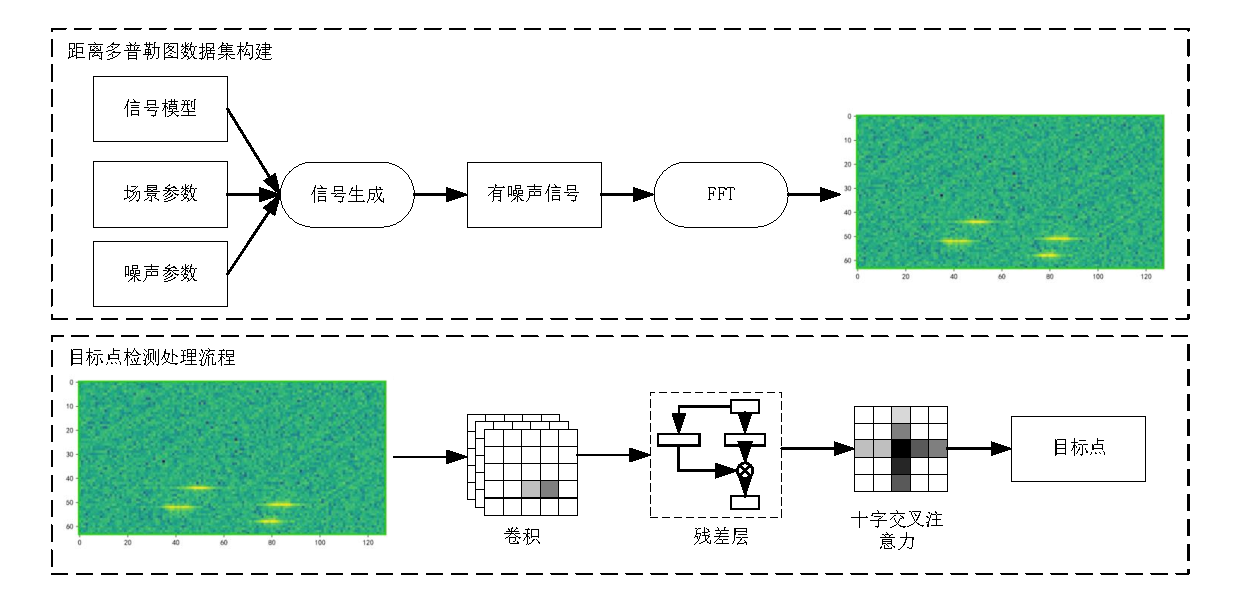
\includegraphics[width=\linewidth]{figures/目标点检测流程.pdf}
	\caption{目标点检测流程}
	\label{fig:目标点检测流程}
\end{figure}


\section{多场景距离多普勒图数据集构建}

\subsection{数据预处理}
一帧的雷达数据含有N个Chrip信号,首先要做的是对每个Chrip做FFT运算,这一步的FFT运算将雷达的回波信号分离成不同距离门限的信号,处理一帧中N个Chrip的信号,并且将得到的频谱以列的方式存储到二维矩阵中。接下来对于每个距离门限的行进行长度为N的FFT运算,测量雷达目标的多普勒频率。经过两次FFT运算得到了一帧距离多普勒图。过程如图\ref{fig:FFT运算}所示。
\begin{figure}[htbp]
	\centering
	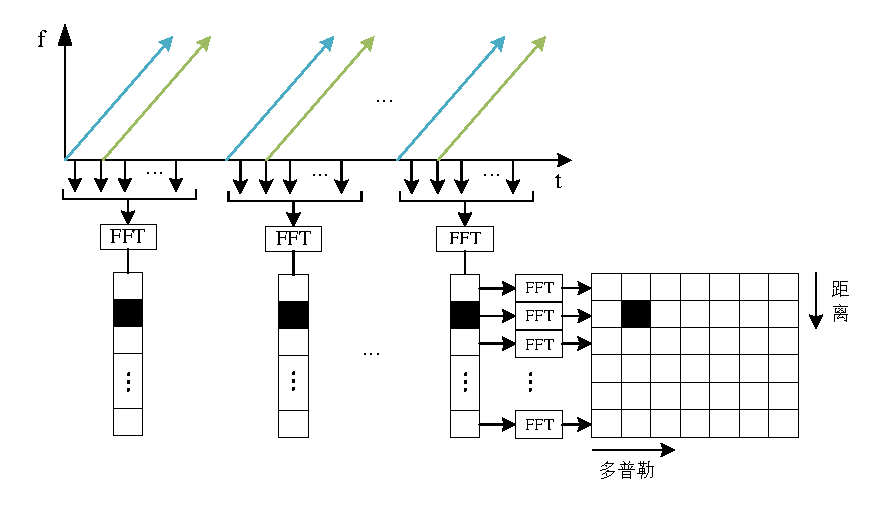
\includegraphics[width=0.8\linewidth]{figures/FFT运算.pdf}
	\caption{FFT运算}
	\label{fig:FFT运算}
\end{figure}


经过二维FFT处理得到的距离多普勒图中存在两种主要类型的干扰:直流分量和静态干扰。直流分量通常是由雷达系统中的直流偏置引起的\cite{gu2000removal},表现为频域中的零频分量。这些直流偏置是由雷达系统中的一些器件,例如放大器和混频器引起的,它们可能会对雷达信号的处理和分析产生影响,从而影响后续的特征提取和分类过程。静态干扰是由场景中静态物体引起的,它在距离多普勒图中表现为速度为0m/s的区域。

除了干扰峰值外,还存在一些峰值与干扰峰值不同,这些峰值对应于移动目标的速度信息。根据多普勒效应,当一个物体相对于雷达运动时,回波信号的频率会发生变化,在速度维上产生频移。通过执行速度维FFT,能够将回波信号在速度维上展开,得到不同速度的目标信息。在距离多普勒图中静态干扰位于速度零轴附近,移动目标对应的峰值位于速度轴两侧。根据峰值的位置能够确定目标的速度方向,峰值的幅度大小反映了目标的速度强度。在噪声和干扰峰值中检测出有效的目标点是毫米波雷达目标点检测的关键问题。
为了获取准确的训练集和测试集,本章使用仿真的方式模仿FMCW雷达发射信号和接受信号的过程,通过建立线性调频连续波模型,发送频率随时间线性变化的波形,模拟FMCW雷达的工作,在收到的回波信号里面加入控制信噪比的高斯噪声。
本章的实验环境如表\ref{实验软硬件环境}所示:

% \begin{table}[htbp]
%     \centering
% 	\caption{实验软硬件环境}
% 	\begin{tblr}{
% 		hline{1,Z} = {1pt},
% 		hline{2},
% 		colspec={cc},
% 	}
% 		软件环境  & 硬件环境 \\
% 		系统:Windows 11   & CPU Intel i7-11700 \\
% 		语言:Python 3.9 MATLAB R2023b    & 内存32G \\
% 		Cuda 11.1 Pytorch 1.10.1   & 硬盘1TB \\
% 		采集工具:mWave Studio   & IWR6843 DCA1000EVM \\
% 	\end{tblr}
% 	\label{实验软硬件环境}
% \end{table}     

\begin{table}[htbp]
	\centering
	\tabcolsep=1cm
	\caption{实验软硬件环境}
	\begin{tabular}{cc}
		\toprule
		软件环境  & 硬件环境 \\
		\midrule
		系统:Windows 11   & CPU Intel i7-11700 \\
		语言:Python 3.9 MATLAB R2023b    & 内存32G \\
		Cuda 11.1 Pytorch 1.10.1   & 硬盘1TB \\
		采集工具:mWave Studio   & IWR6843 DCA1000EVM \\
		\bottomrule
	\end{tabular}
	\label{实验软硬件环境}
\end{table}

\subsection{信号模型建立} \label{信号模型建立}
因为FMCW雷达发射信号的频率是一个随时间变化的线性函数,如图\ref{chrip}所示。发送信号的模型\cite{DBLP:journals/tcas/GerstmairMOSH18}可以使用公式\eqref{eq:发送信号}表示。公式中$signal(t)$为当前发射的信号,$A$为信号的幅度,$S$为Chrip信号随时间线性变化的斜率,$T$为当前帧的周期,$f_0$为载频。
\begin{equation}
	\label{eq:发送信号}
	S_t(t) = A \cos\big(2\pi (f_0t+\frac{St^2}{2}) + \phi_0 \big), t \in [0,T]
\end{equation}
由此可得,FMCW雷达发送信号模型的相位可以用公式\eqref{eq:发送相位}表示:
\begin{equation}
	\label{eq:发送相位}
	P_t(t) = 2\pi (f_0t+\frac{St^2}{2})+ \phi_0, t \in [0,T]
\end{equation}
经过每个时间间隔$\tau$,都会发送一个Chrip信号。利用多个Chirp来测量目标的速度。

\begin{figure}[htbp]
	\centering
	\subcaptionbox{幅度变化}{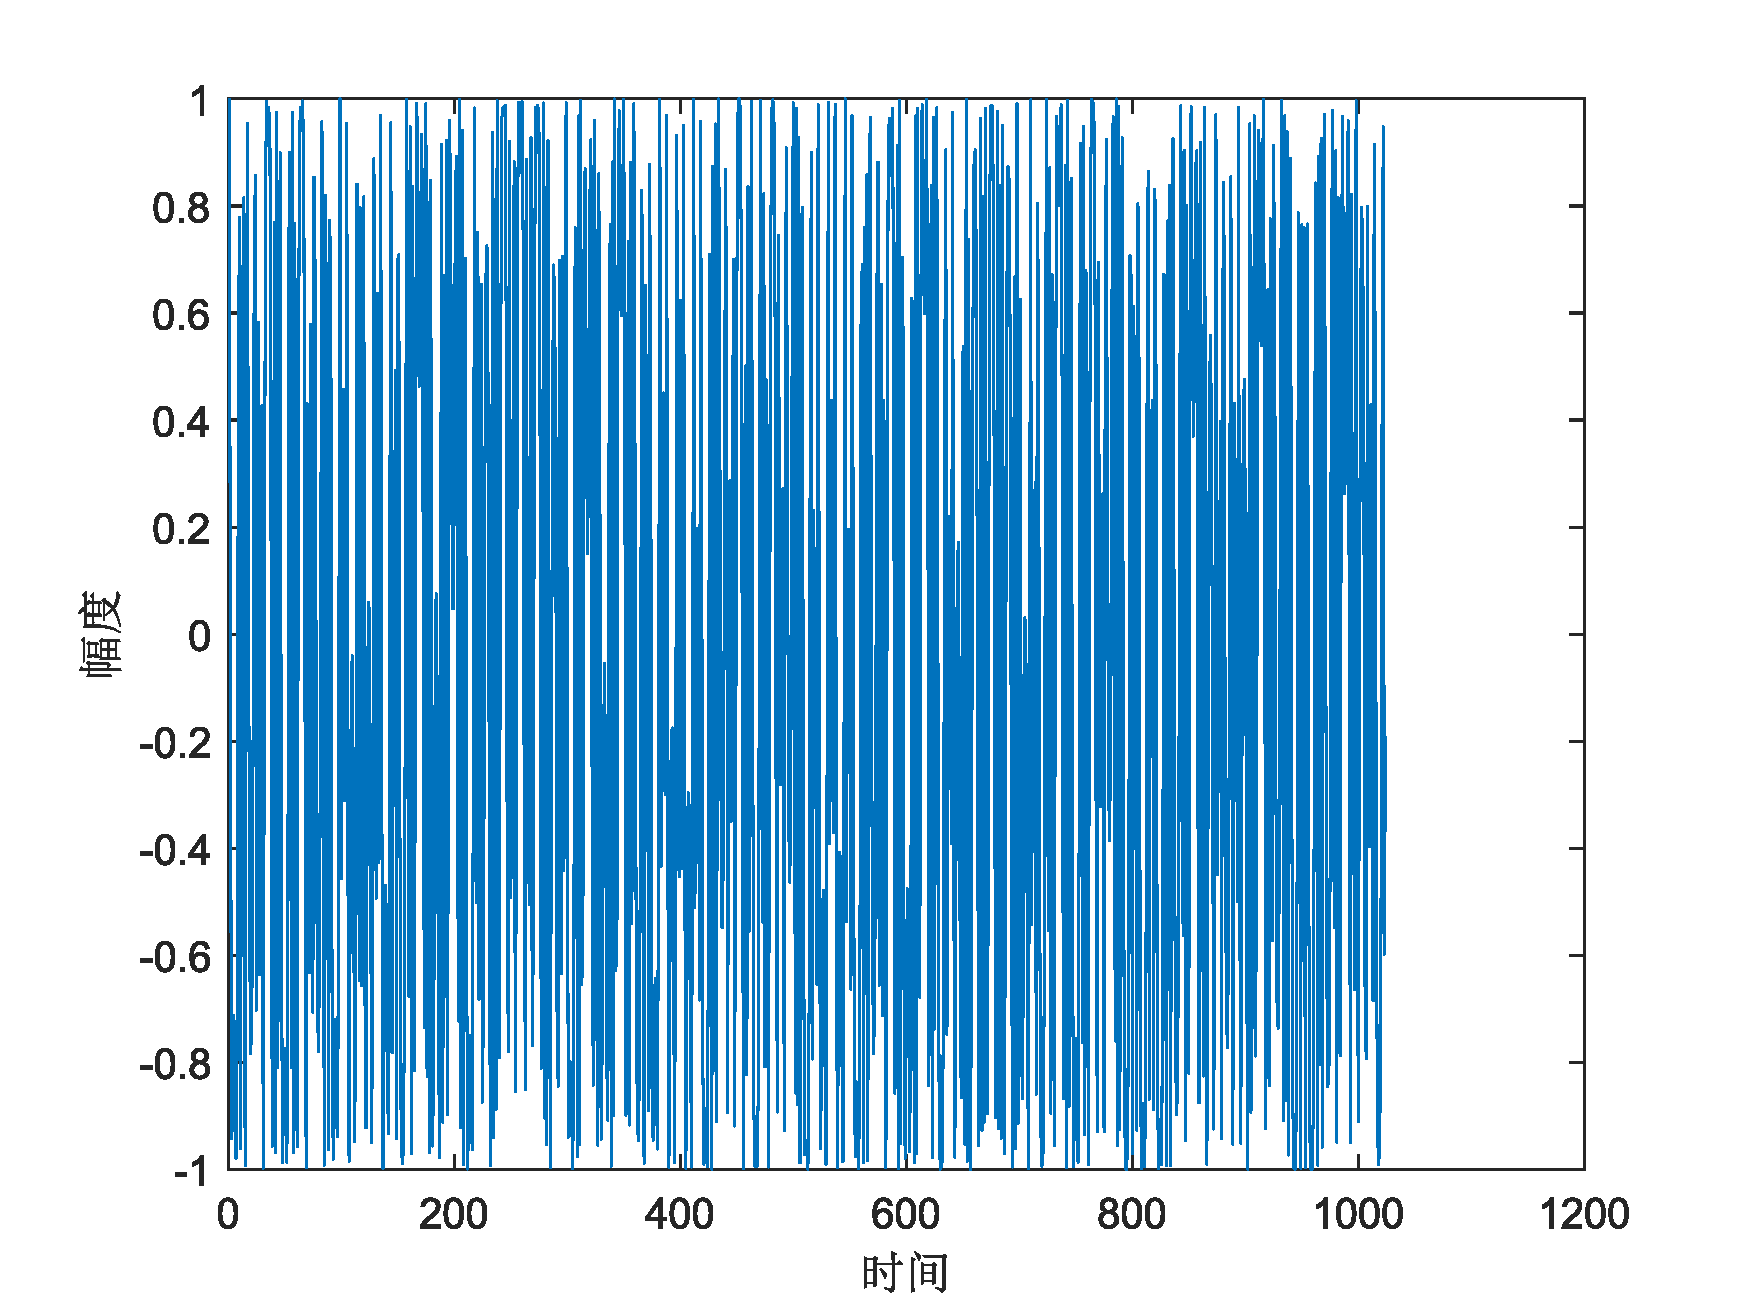
\includegraphics[width = 0.45\textwidth]{figures/发射信号幅度.pdf}}
	\subcaptionbox{频率变化}{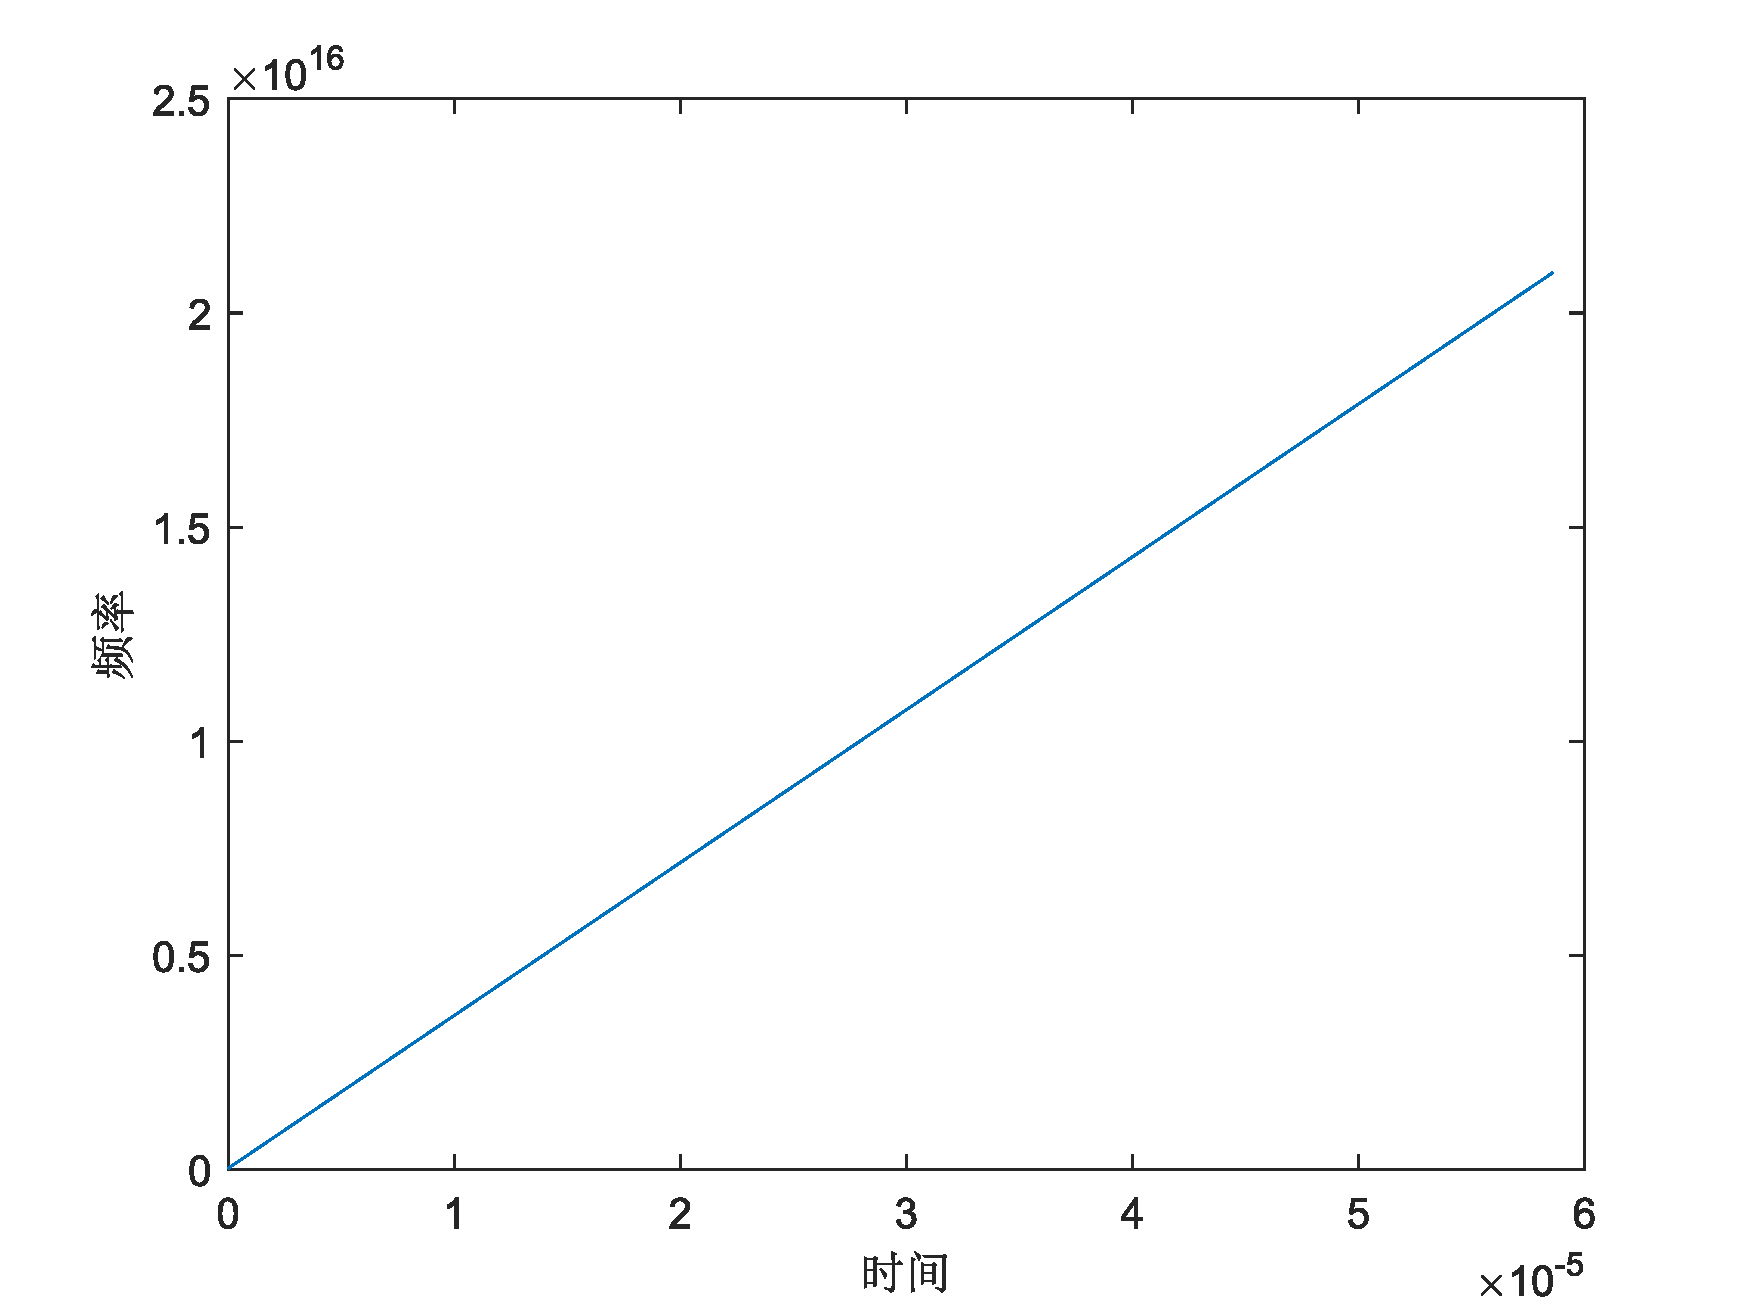
\includegraphics[width = 0.45\textwidth]{figures/发射信号频率.pdf}}
	\caption{发送信号时频域图}
	\label{fig:发送信号时频域图}
\end{figure}

已知电磁波的传输速度为光速$c$,假设测量目标与雷达的距离为$R$,则雷达收到回波信号的延迟为$\tau=\frac{2R}{c}$,$K$为雷达接收到信号的衰减系数\cite{matrosov2008assessment}。因此由公式\eqref{eq:发送信号}可知,接收到的回波信号的模型如公式\eqref{eq:接受信号}所示:
\begin{equation}
	\label{eq:接受信号}
	S_r(t) = KA \cos\big(2\pi (f_0(t - \tau)+\frac{S(t-\tau)^2}{2}) + \phi_0 \big), t \in [0,T]
\end{equation}
由公式\eqref{eq:发送相位}和\eqref{eq:接受信号}可得,回波信号的相位模型为:
\begin{equation}
	\label{eq:接收相位}
	P_r(t) = 2\pi \big(f_0(t-\tau)+\frac{S(t-\tau)^2}{2}\big)+ \phi_0, t\in [0,T]
\end{equation}
将接收到的回波信号$S_r(t)$与发送信号$S_t(t)$进行混频后,经过低通滤波就可以得到一个差频信号,这个信号是单一频率的正弦波。差频信号的相位表达式如下:
\begin{equation}
	\label{eq:中频}
	\begin{split}
		P_t(t) - P_r(t) &= \Big(2\pi(f_0t+\frac{St^2}{2})+\phi_0\Big) - \Big(2\pi \big(f_0(t-\tau)+\frac{S(t-\tau)^2}{2}\big)+ \phi_0\Big) , t\in [0,T]\\
		&=2\pi f_0\tau + 2\pi S \tau t - \pi S \tau^2
	\end{split}
\end{equation}
为了模拟真实的场景,需要在回波信号中添加指定信噪比(Signal to Noise Ratio,SNR)的高斯噪声\cite{luisier2010image}。回波信号的模型函数公式\eqref{eq:接受信号}是已知的,在已知原始干净信号后,SNR的计算公式如\eqref{eq:SNR}所示:
\begin{equation}
	\label{eq:SNR}
	SNR = 10\log10(signalPower / Power(noisedSignal- Signal))
\end{equation}

因此添加一个已知SNR的噪声步骤如下:
\par
(1)计算原始信号的平均功率:
\begin{equation}
	signalPower = sum(abs(S_r)^2) / length(S_r)
\end{equation}

(2)将平均功率转为dB:
\begin{equation}
	signalPowerdB = 10\log10(signalPower)
\end{equation}
\par
(3)计算噪声的平均功率(dB):
\begin{equation}
	noisePowerdB = signalPowerdB -SNR
\end{equation}
\par
(4)计算噪声的平均功率:
\begin{equation}
noisePower = 10^{(noisePowerdB /10)}
\end{equation}
\par
(5)最后得到需要添加的噪声为:
\begin{equation}
noise = \sqrt{noisePower}*randn(length(S_r),1)
\end{equation}
\subsection{训练数据生成} \label{训练数据生成}
为了得到与距离多普勒图目标点对应的真实标签值,本节采用仿真环境建立数据集。由于不同的噪声水平和目标数量会影响到特征提取的成功率,为了提高模型的泛化能力,本节根据不同动目标速度生成回波信号并且根据不同的SNR生成并添加噪声,使用添加噪声后的混合信号成距离多普勒图。使用距离多普勒图作为输入数据,动目标图作为标签生成训练数据。
单目标距离多普勒图如图\ref{fig:单目标距离多普勒图}所示,多目标距离多普勒图如图\ref{fig:多目标距离多普勒图}所示。

仿真环境的参数设置如表\ref{仿真环境参数}所示,其中SNR的取值涵盖了从低信噪比到高信噪比的范围,动目标速度为从20-60m/s随机生成。
\begin{figure}[htbp]
	\centering
	\subcaptionbox{距离多普勒}{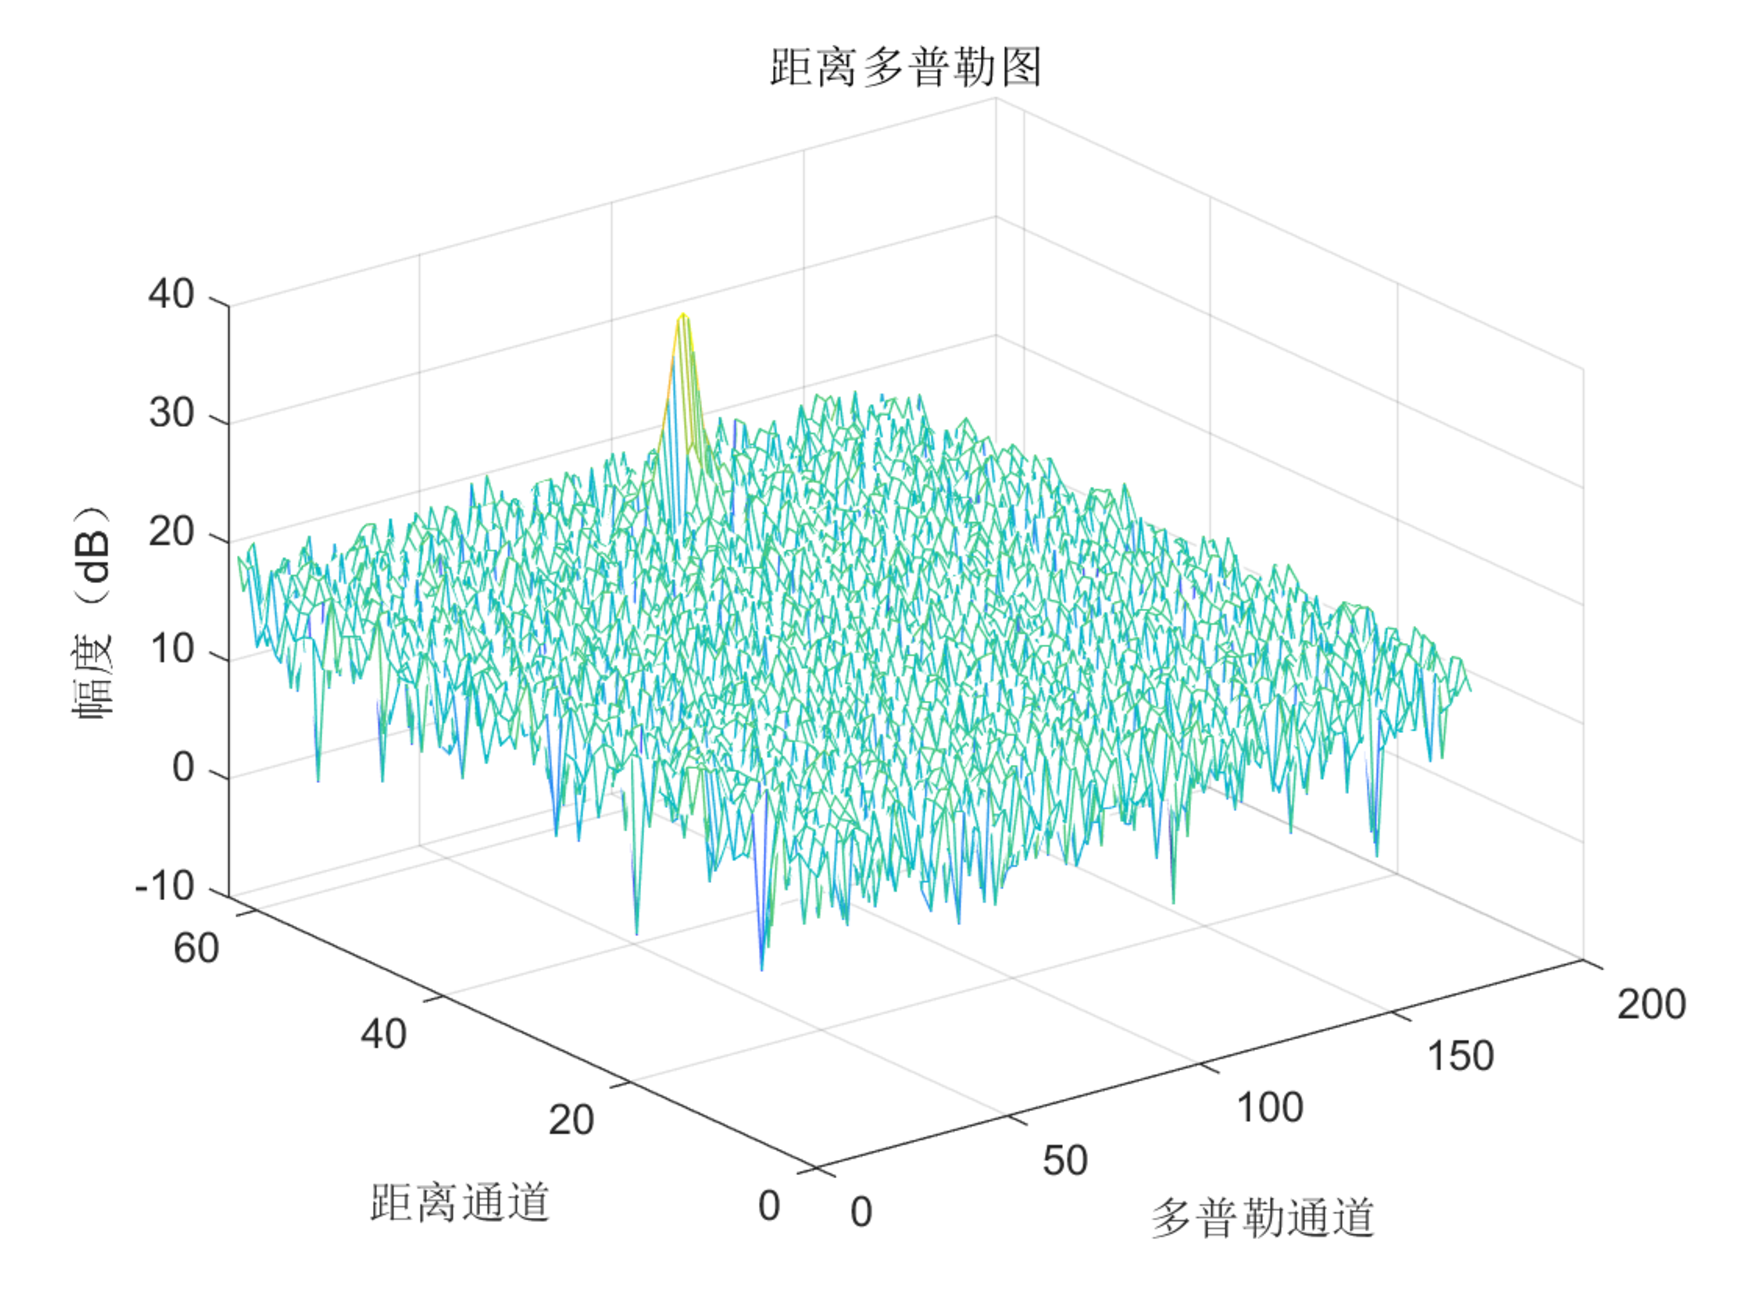
\includegraphics[width = 0.4\textwidth]{figures/1目标距离多普勒.pdf}}
	\subcaptionbox{动目标图}{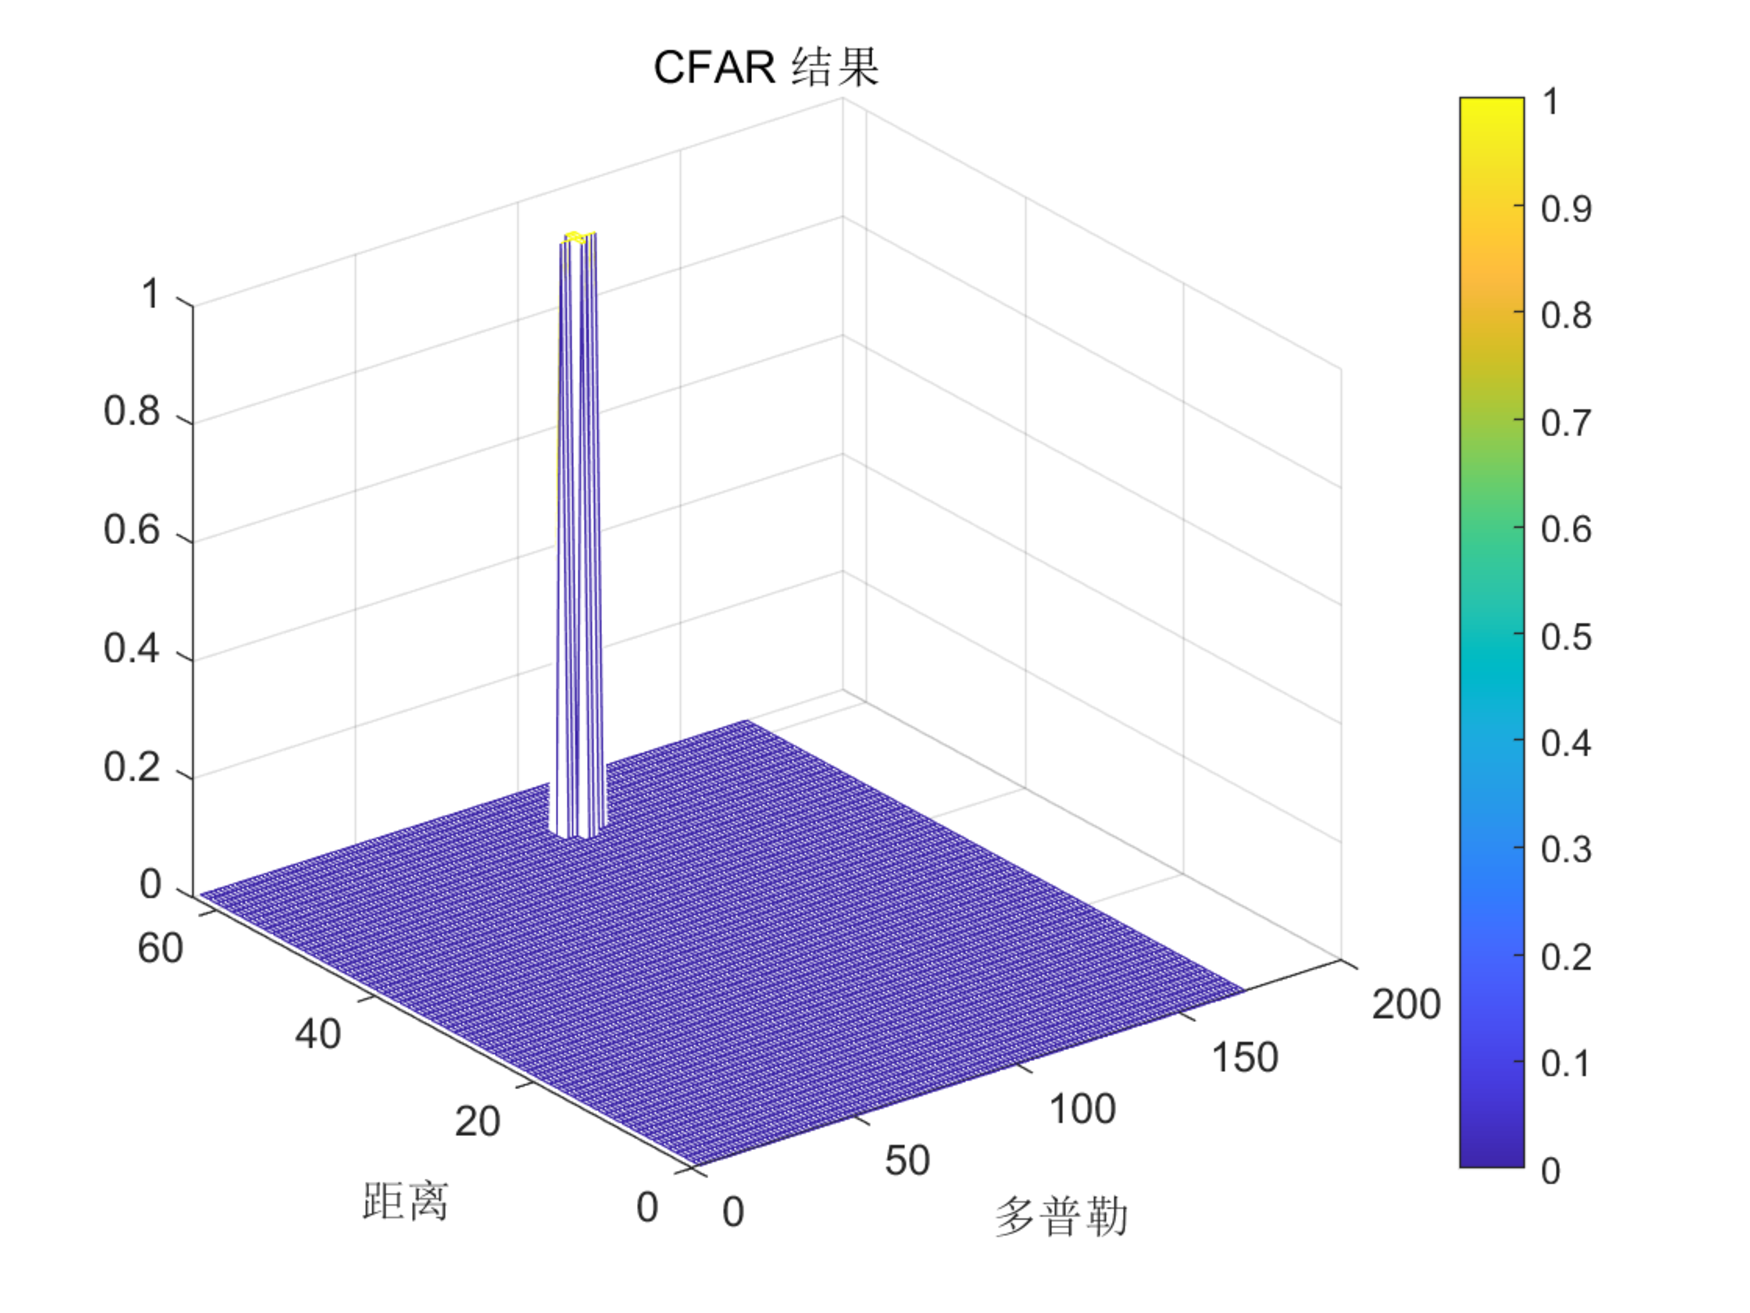
\includegraphics[width = 0.4\textwidth]{figures/1目标CFAR.pdf}}
	\caption{单目标距离多普勒图}
	\label{fig:单目标距离多普勒图}
\end{figure}
\begin{figure}[htbp]
	\centering
	\subcaptionbox{二目标距离多普勒}{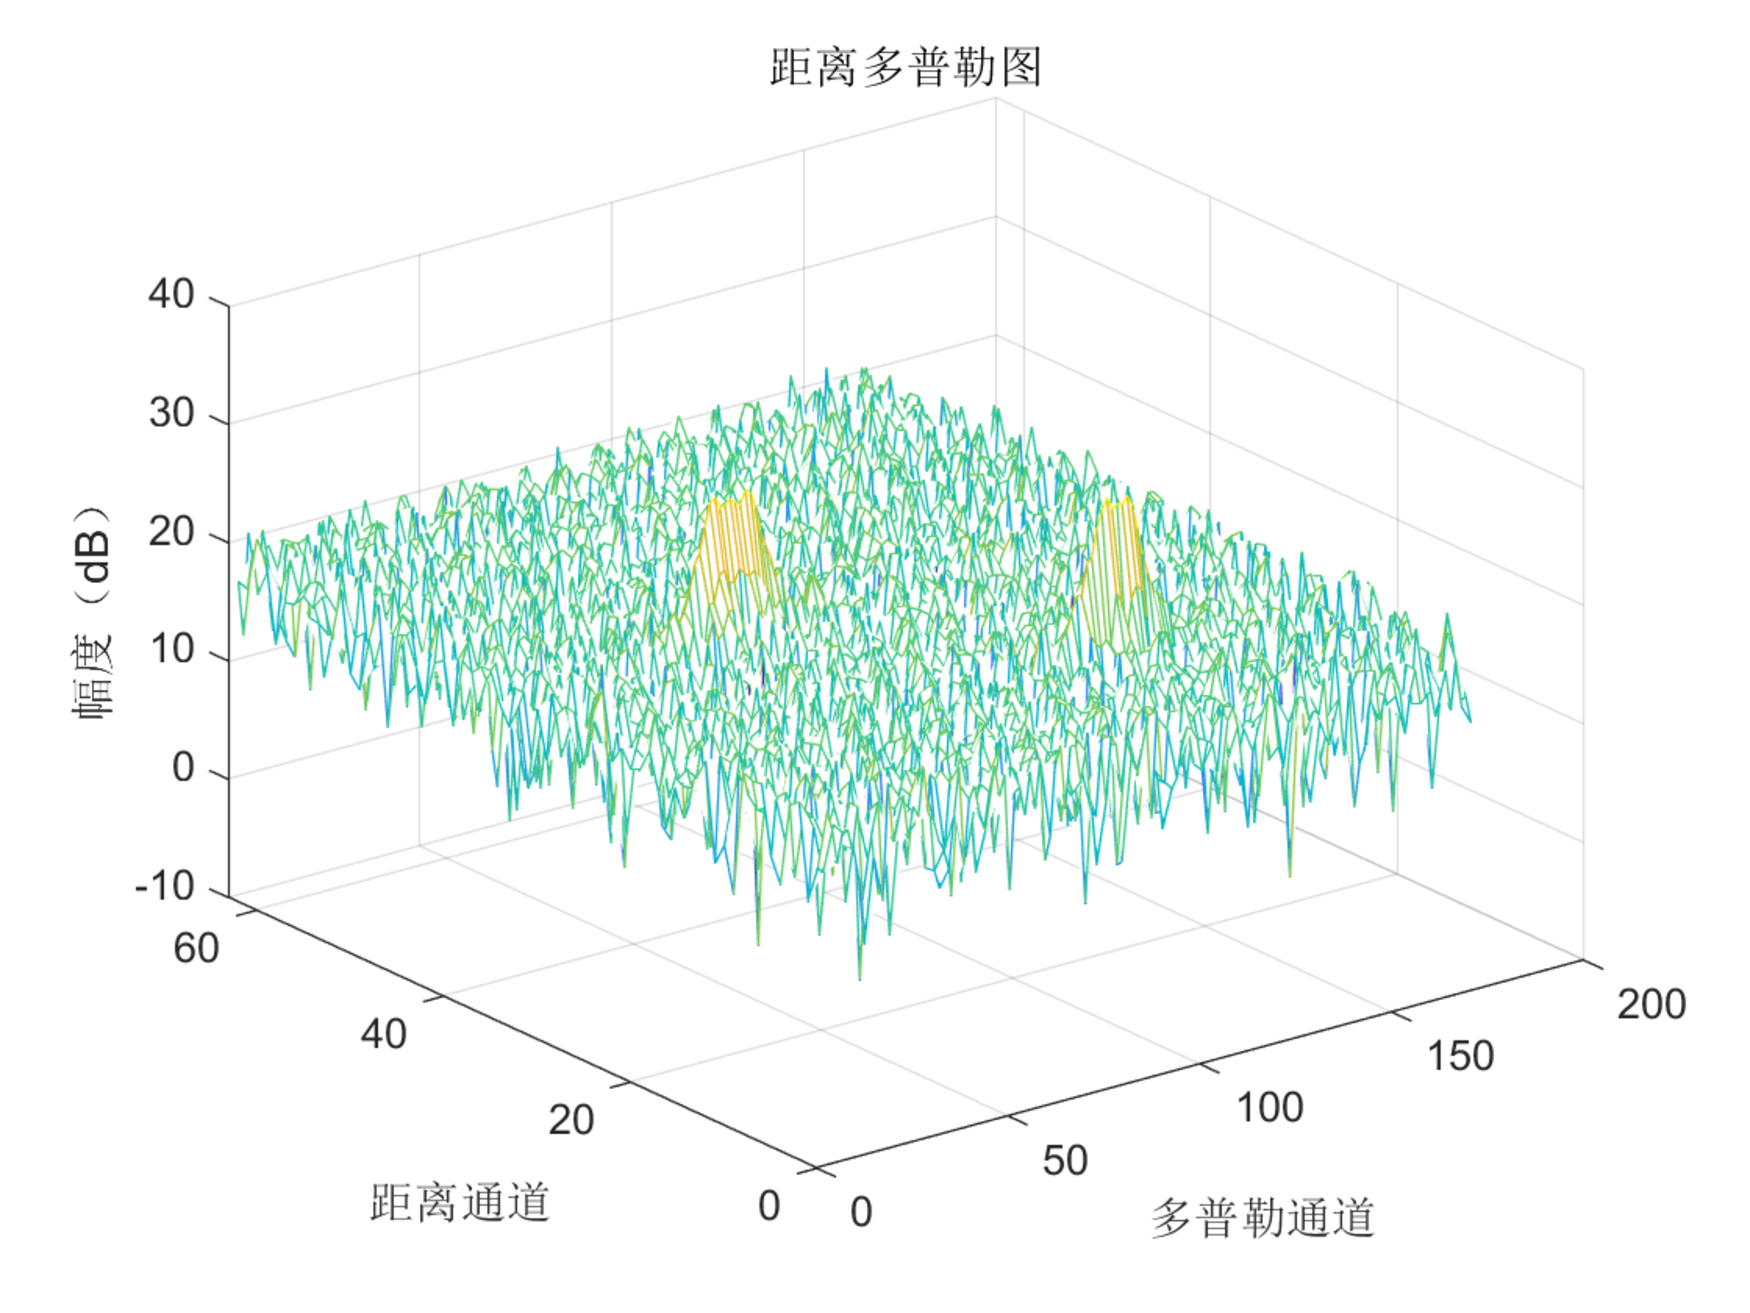
\includegraphics[width = 0.4\textwidth]{figures/2目标距离多普勒.pdf}}
	\subcaptionbox{三目标动目标图}{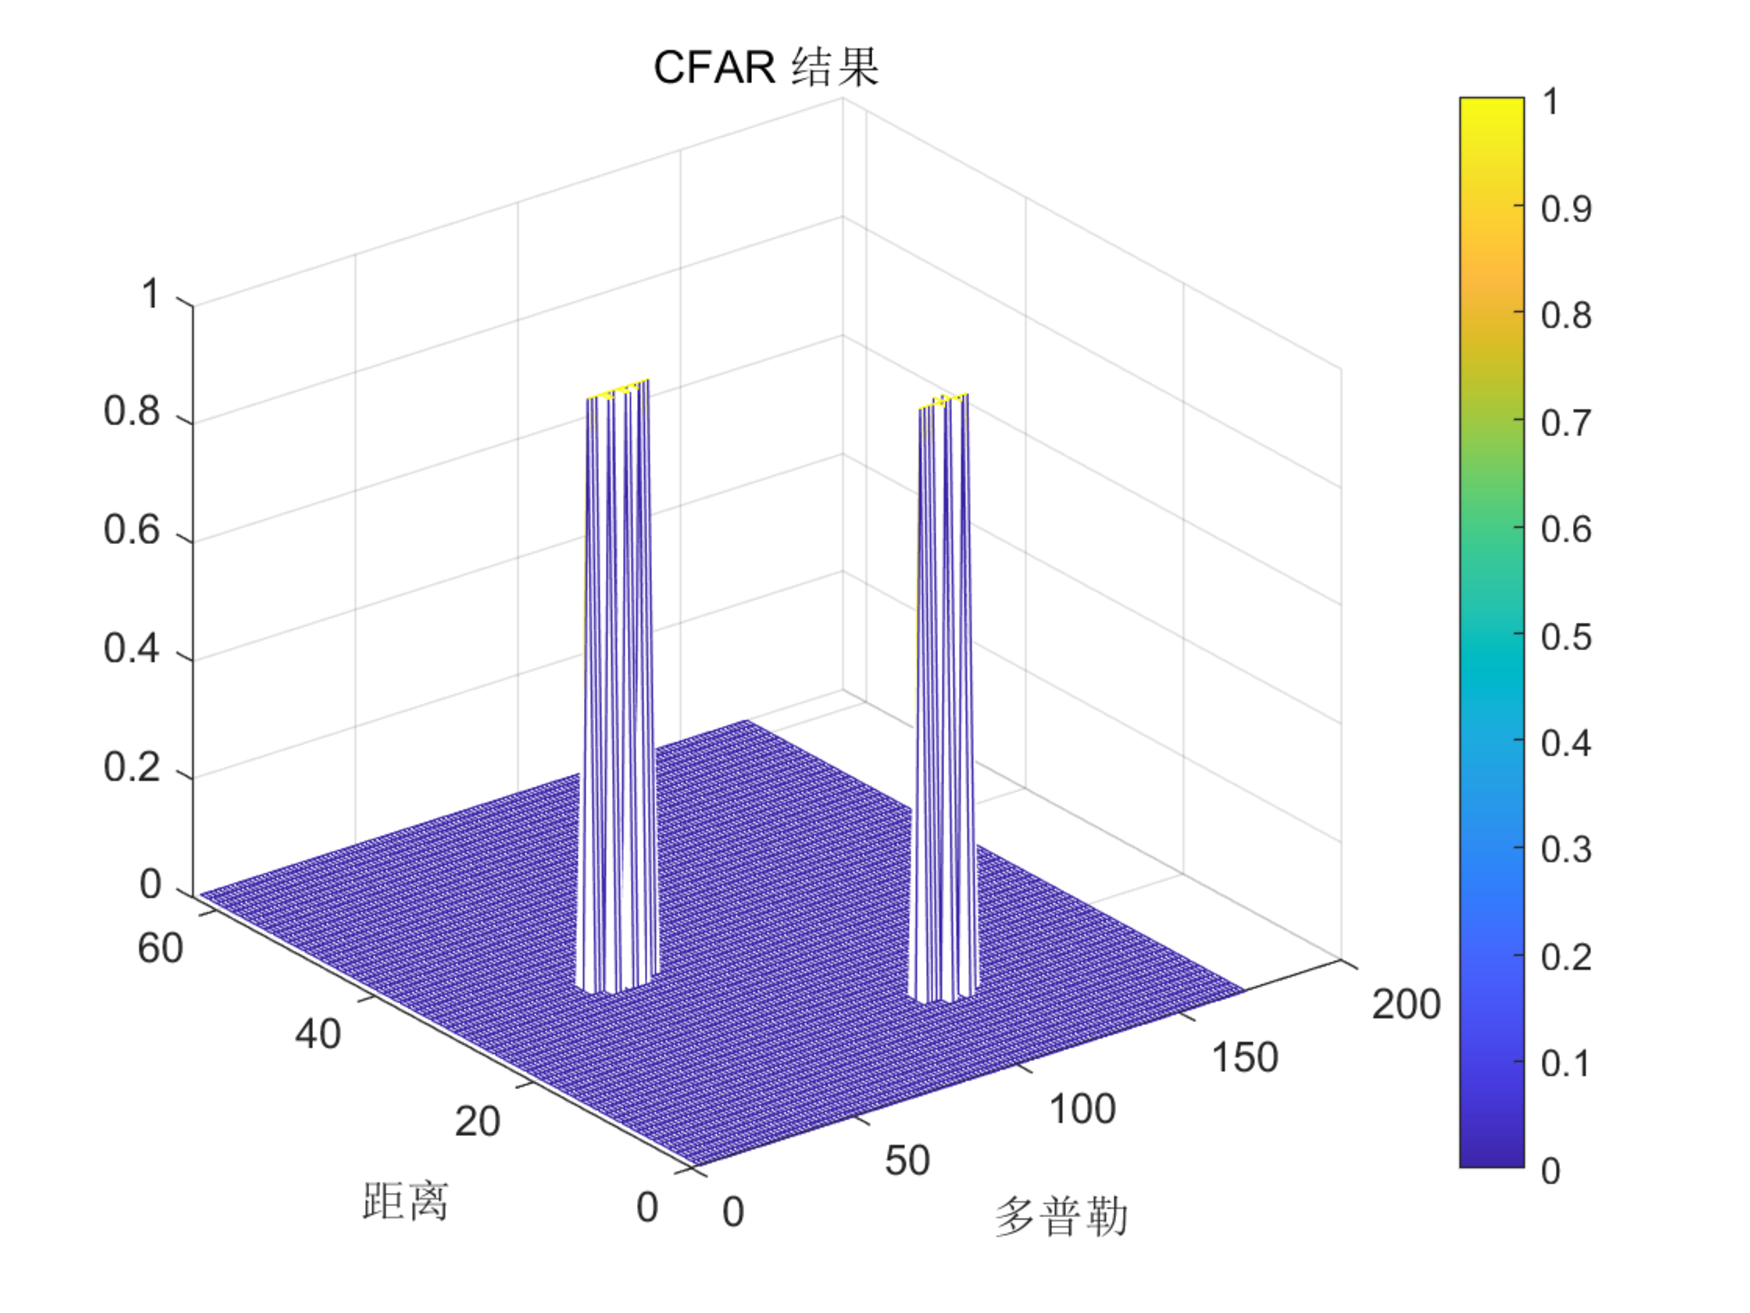
\includegraphics[width = 0.4\textwidth]{figures/2目标CFAR.pdf}}
	\subcaptionbox{三目标距离多普勒}{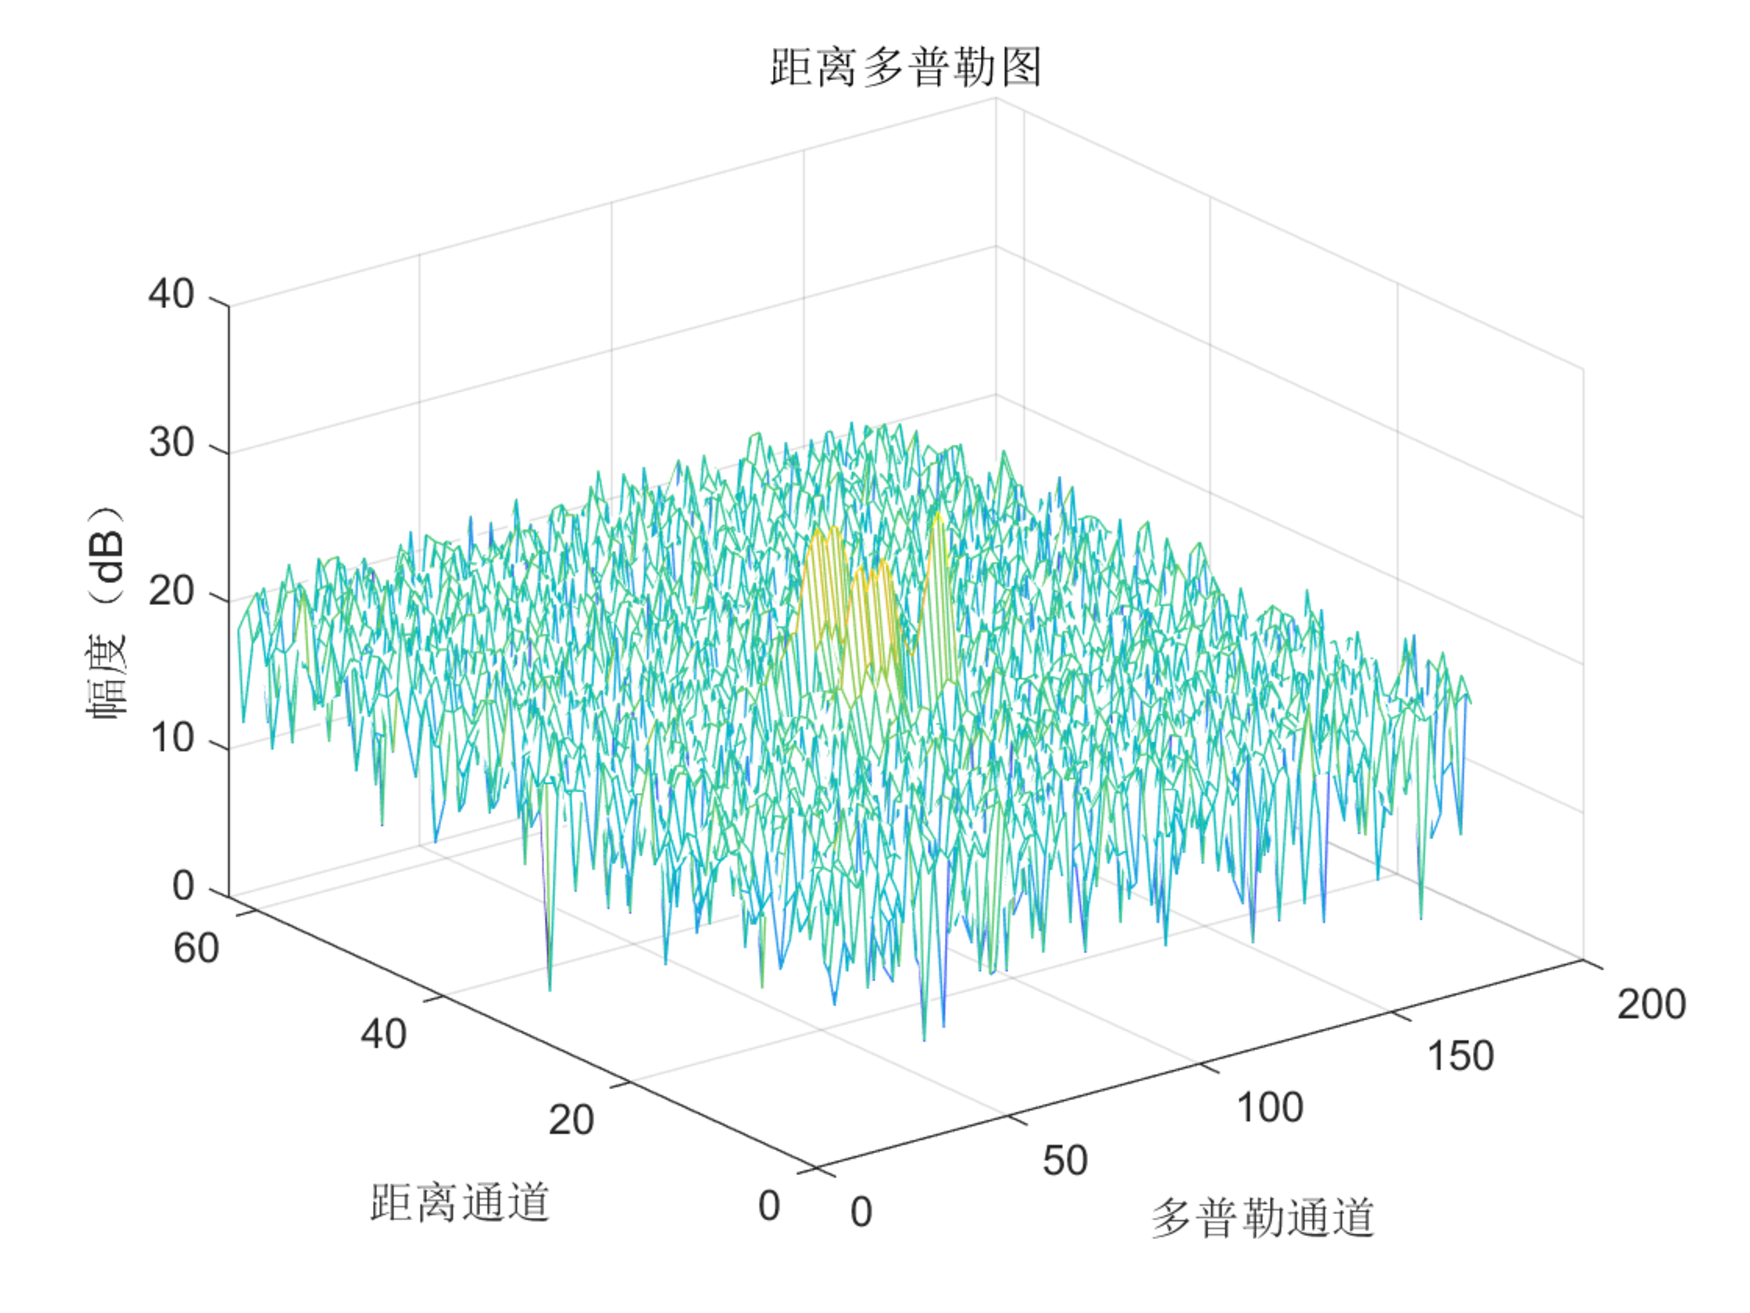
\includegraphics[width = 0.4\textwidth]{figures/3目标距离多普勒.pdf}}
	\subcaptionbox{三目标动目标图}{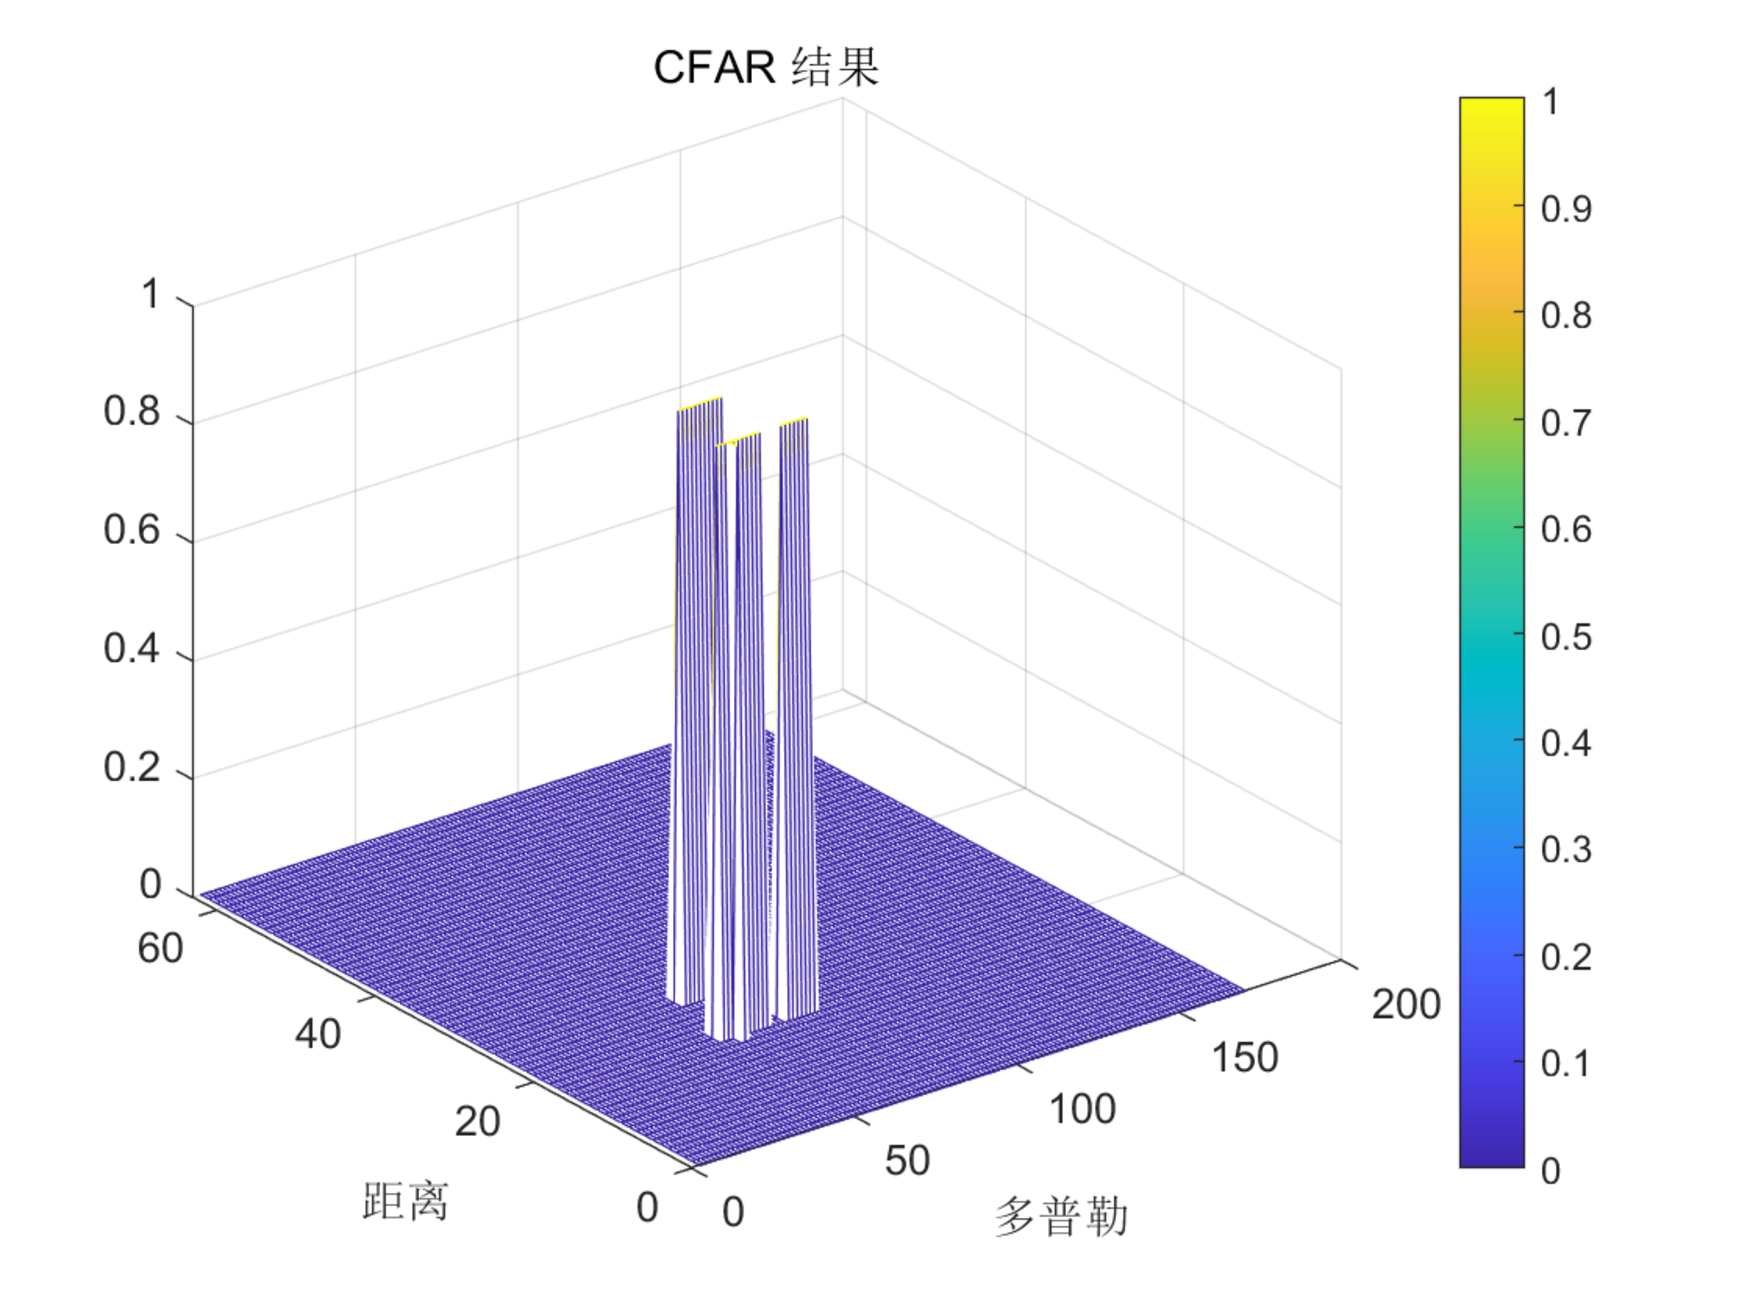
\includegraphics[width = 0.4\textwidth]{figures/3目标CFAR.pdf}}
	\caption{多目标距离多普勒图}
	\label{fig:多目标距离多普勒图}
\end{figure}

\begin{table}[htbp]
	\centering
	\caption{仿真环境参数}
	\begin{tabular}{cccc}
		\toprule
		\diagbox{SNR}{动目标数量} & 1 & 2 & 3 \\
		\midrule
		20dB & 20dB,1目标& 20dB,2目标& 20dB,3目标\\
		25dB & 25dB,1目标& 25dB,2目标& 25dB,3目标\\
		30dB & 30dB,1目标& 30dB,2目标& 30dB,3目标\\
		35dB & 35dB,1目标& 35dB,2目标& 35dB,3目标\\
		\bottomrule
	\end{tabular}
	\label{仿真环境参数}
\end{table}
\begin{table}[htbp]
	\centering
	\tabcolsep=1cm
	\caption{雷达参数表}
	\begin{tabular}{cc}
		\toprule
		参数 & 数值 \\
		\midrule
		发射天线 & 4  \\
		接收天线 &3   \\
		ADC采样点数 & 128  \\
		开始频率 & 60GHz   \\
		空闲时间 & 10ns  \\
		每帧Chrip数 & 128 \\
		\bottomrule
	\end{tabular}
	\label{雷达参数表}
\end{table}

\subsection{实验数据采集} \label{实验数据采集}
为了验证在实际环境中效果,使用德州仪器IWR-6843毫米波雷达采集了多个环境中的数据。
搭建的实验环境为,使用DCA1000EVM数据采集板通过网口将ADC采样的RAW数据传输到PC上。数据收集的场地为开阔室内和走廊,雷达高度为1.5m。雷达参数配置如表所示,雷达设备如图\ref{fig:实验设备}所示。

\begin{figure}[htbp]
	\centering
	\subcaptionbox{正面}{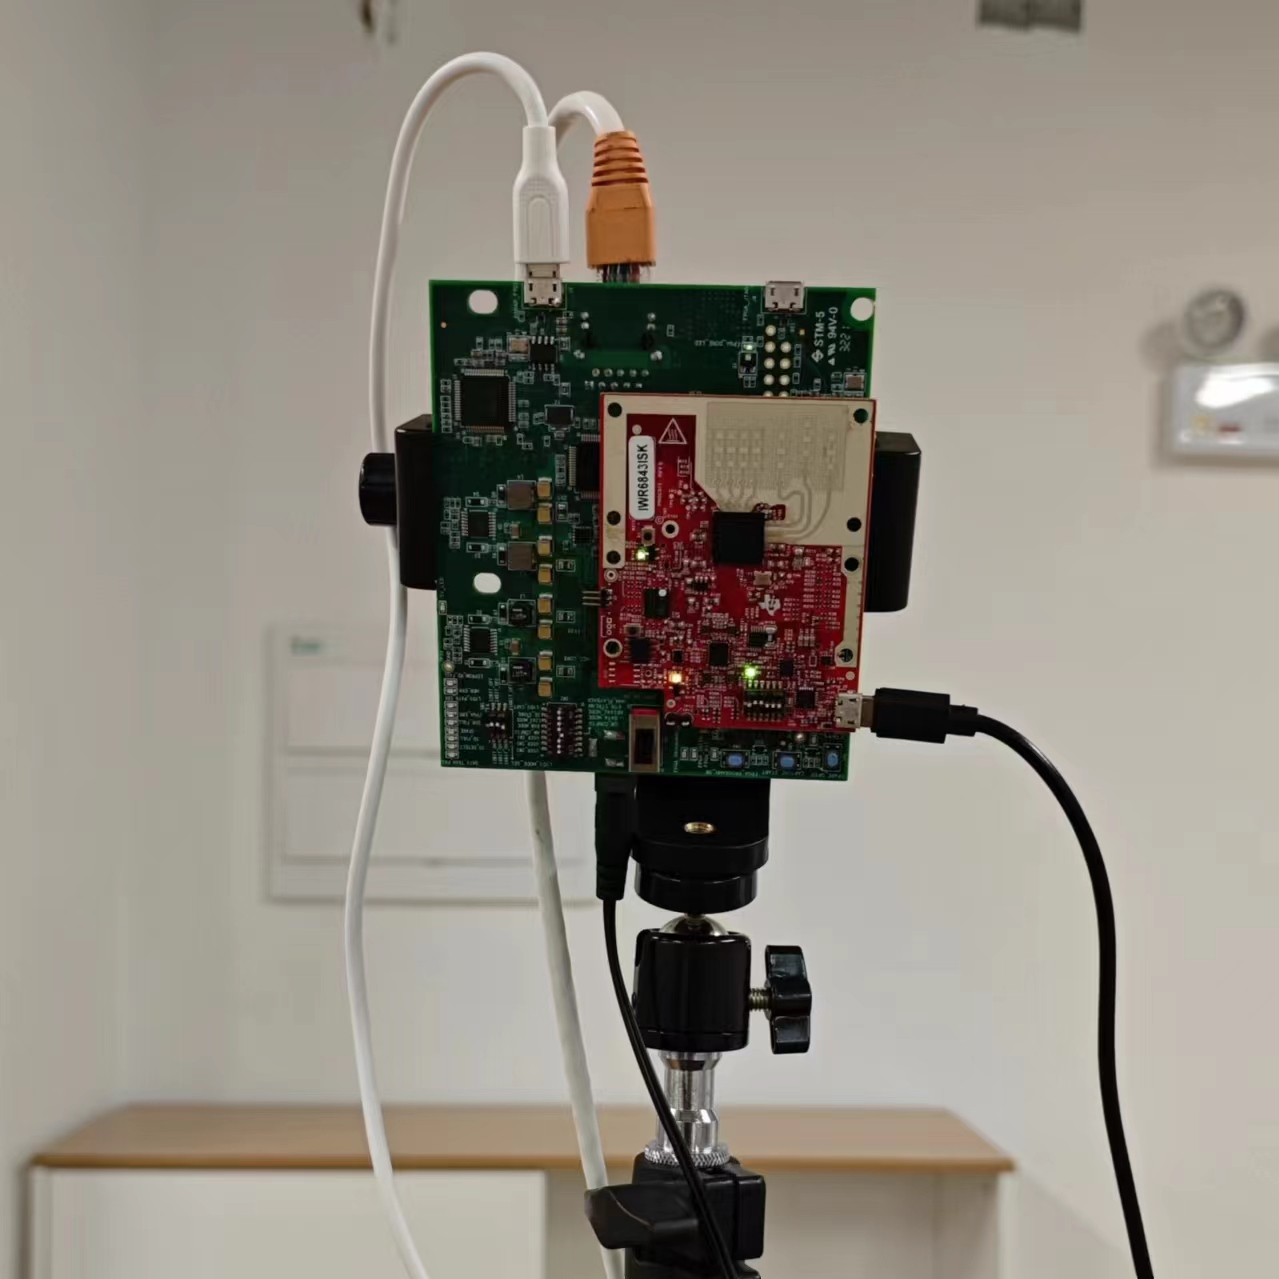
\includegraphics[width = 0.4\textwidth]{images/正面.jpg}}
	\subcaptionbox{背面}{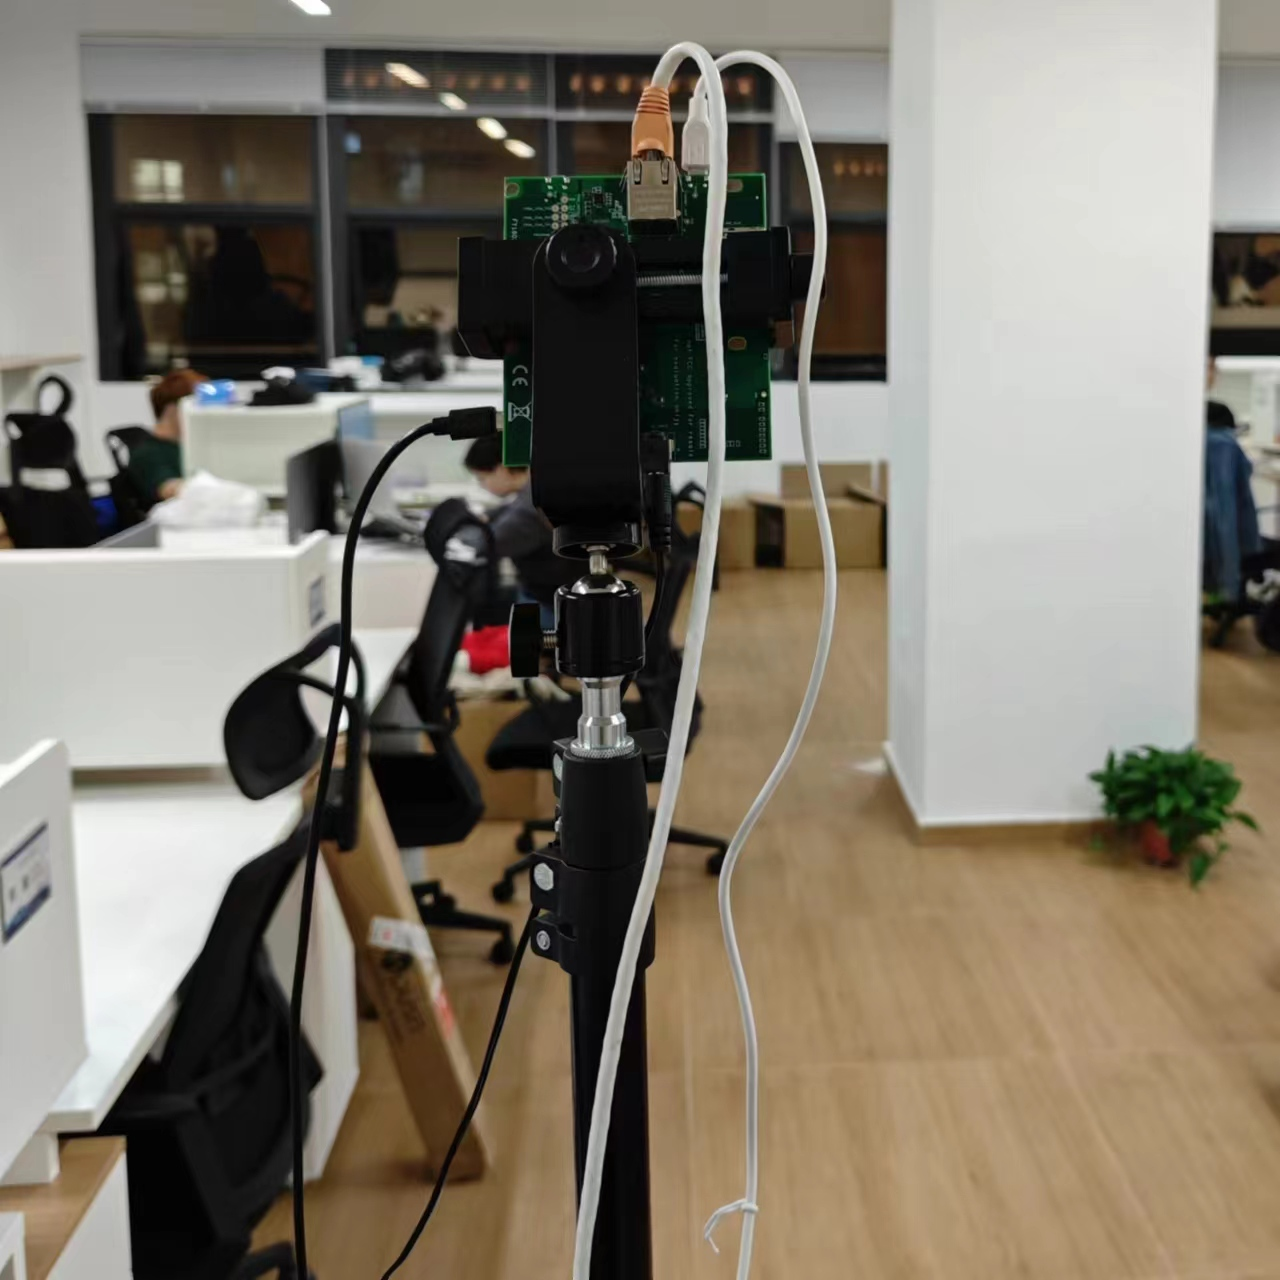
\includegraphics[width = 0.4\textwidth]{images/背面.jpg}}
	\caption{IWR6843毫米波雷达}
	\label{fig:实验设备}
\end{figure}


每个地点不同的人数采集100组数据,共计采集6000组数据。经过FFT后得到的距离多普勒图大小为$96 \times 128$,室内与室外数据采集参数如表\ref{采集数据参数}所示。
\begin{table}[htbp]
	\caption{采集数据参数}
	\begin{subtable}{.4\linewidth}
		\centering
		\caption{单人采集数据}
		\begin{tabular}{ccc}
			\toprule
		    人员 & 移动速度 & 样本数量  \\
			\midrule
			1号 &2 m/s & 100 \\
			2号 &1 m/s & 100 \\
			3号 &3 m/s & 100  \\
			\bottomrule
		\end{tabular}
	\end{subtable}
	\begin{subtable}{.4\linewidth}
		\centering
		\caption{多人采集数据}
		\begin{tabular}{ccc}
			\toprule
			人数 & 移动速度 & 样本数量  \\
			\midrule
			2人 & 1 m/s,2 m/s& 100 \\
			3人 & 1 m/s,2 m/s,3 m/s & 100  \\
			\bottomrule
		\end{tabular}
	\end{subtable}
	\label{采集数据参数}
\end{table}

\section{距离多普勒图目标点检测方案}

\subsection{基于残差网络的全图特征提取}
残差块模型设计如图\ref{fig:ResidualNet}所示,在每个残差块中,使用二维卷积提取特征,使用$3\times3$的卷积核提取距离多普勒图中的空间局部相关性。网络由四个残差块组成,在残差块后接展平层和两层线性层。

(1)残差块设计。每个残差块包含两个$3\times3$卷积层,两个Batch Norm层,两个Relu层和一个$1\times1$的卷积层用于从输入到输出的跳跃连接。
\begin{figure}[htbp]
	\centering
	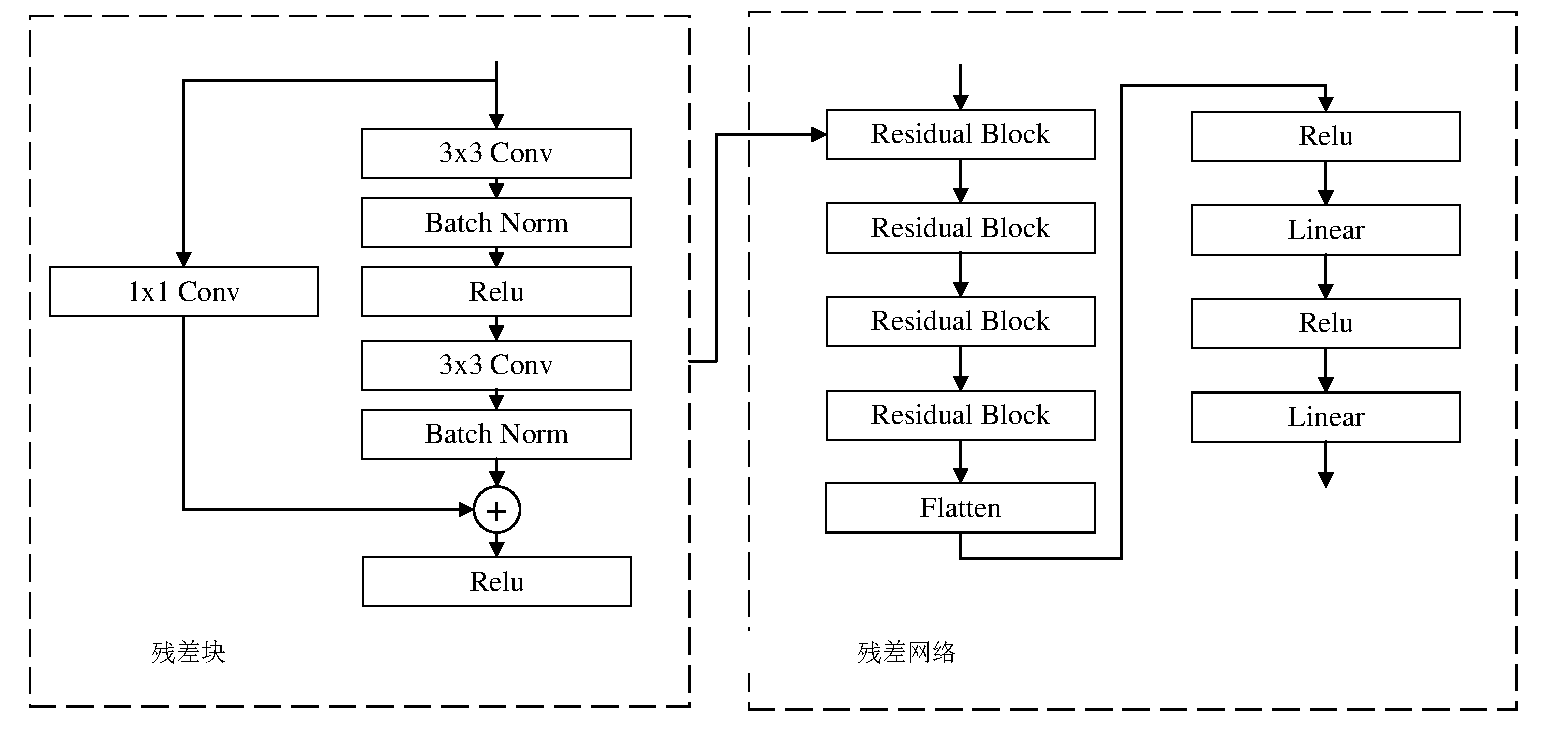
\includegraphics[width=\linewidth]{figures/残差网络.pdf}
	\caption{残差网络模型设计}
	\label{fig:ResidualNet}
\end{figure}
当前输入的特征$X$的维度为$(B,1,H,W)$,其中$B$为Batch大小,1为特征通道数,$H$和$W$为输入距离多普勒图的长和宽。输入特征经过两次卷积和两次归一化后,特征$Y$维度变为$(B,64,H,W)$,为了保证网络加深后输入特征不丢失,在残差块输出之前加入原始输入数据。因此时$X$的维度与$Y$的维度不匹配,所以需要$1\times1$的卷积层,将$X$的维度变为$(B,64,H,W)$。残差块输出的$Y=Y+X$。残差块的设置如表\ref{残差块参数设置}所示。

\begin{table}[htbp]
	\centering
	\tabcolsep=3mm
	\caption{残差网络参数设置}
	\begin{tabular}{ccccccc}
		\toprule
		层  & 核大小 & 输入通道 & 输出通道 & 步数 & 填充 & 输出 \\
		\midrule
		Conv & 3 \times 3 & -- & -- & -- & -- & -- \\
		ResidualBlock &3 \times 3 & 1 & 16 & 1 & 1 & B $\times$ 16 $\times$ H $\times$ W \\
		ResidualBlock &3 \times 3 & 16 & 32 & 1 & 1 & B $\times$ 32 $\times$ H $\times$ W \\
		ResidualBlock &3 \times 3 & 32 & 8 & 1 & 1 & B $\times$ 8 $\times$ H $\times$ W \\
		ResidualBlock &3 \times 3 & 8 & 1 & 1 & 1 & B $\times$ 1 $\times$ H $\times$ W \\
		Criss-Cross Attention & -- & 1 & 1 & -- & -- & B $\times$ 8 $\times$ H $\times$ W \\
		Skip Conn & 1 \times 1 & in & out & -- & -- & B $\times$ out $\times$ H $\times$ W \\
		Flatten & -- & -- & -- & -- & -- & B \times (H $\times$ W) \\
		FC & -- &  (H $\times$ W) & 256  & -- & -- & B \times 256 \\
		FC & -- &  256 & 512  & -- & -- & B \times 512 \\
		FC & -- & 512 & (H $\times$ W)  & -- & -- & B \times (H $\times$ W) \\
		\bottomrule
	\end{tabular}
	\label{残差块参数设置}
\end{table}

(2)模型网络设计。RA-CFAR采用了改造后的残差块做为基础,搭建了神经网络模型。使用四个残差块叠加对特征先升维后降维的方式实现距离多普勒图中噪声特征的提取。实验中对比使用五个残差块将特征维度升到64维后降维的方案,训练时间大幅增加而精确度无明显提升,因此采用四个残差块叠加。每个残差块的卷积层之后都使用了批归一化层和Relu层用来缓解网络梯消失的问题,残差块的卷积层中使用$3\times3$的卷积核大小避免丢失距离多普勒图中小范围特征。为减少空间信息的丢失,残差块中的卷积层在提升特征通道数后保留了原图尺寸。为使每个残差块输入与输出维度匹配,使用$1\times1$的卷积核匹配输入输出维度。在残差块之后使用自适应池化层在后两个维度上进行池化。池化之后使用展平层将特征数据展平为一维向量,输入到二层全连接层得到最终的输出结果。

\subsection{基于十字交叉注意力机制的目标点检测}
为了捕捉距离多普勒图中目标点区域的空间位置的关联性,在残差网络模块之后引入十字交叉注意力机制检测目标点。从距离多普勒图中识别目标的任务近似于从图像中分离出目标与背景的任务。注意力机制可以改善目标检测任务中对目标区域的定位和识别能力。通过在图像中的不同位置计算注意力权重,模型可以更好地理解目标与背景之间的关系,并且更准确地定位和识别目标。由于距离多普勒图是从距离维和多普勒维两次FFT运算得到,其目标点单元所在行和列的幅度水平反应了目标点的位置信息。因此,引入十字交叉注意力机制在每个单元的行和列上进行自注意力计算,有效评估目标点的位置信息。

在残差神经网络之后引入十字交叉注意力机制的工作过程分为如下几个步骤:
\par
(1)将残差神经网络提取得到的特征图中每个单元格所在的行和列分别作为自注意力机制的输入,构建查询、键和数值的表示。在经过残差块的特征提取后,获取的特征是与原输入距离多普勒图尺寸相同的但是被展平成一维的特征向量,记此向量为$D$,将其经过$1\times1$卷积后作为自注意力机制特征向量。表示为:
\begin{equation}
	Q=Conv(D)
\end{equation}
其中$Q$是根据输入特征构建的查询向量。通过计算输入查询向量与键值向量的相关性得到输出向量。
\par
(2)获取每个单元格的归一化权重。取$Q$中一单元格的特征通道值$q=Q(i,j)$,$Q$的尺寸为$(1,H,W)$,$H$和$W$分别为距离多普勒图的高和宽,$i$和$j$分别为单元格的行和列。取$K$中与$q$同行和列的所有单元格的特征通道值$k$,交叉位置只取一次。得到$k$的尺寸为$(1,H+W-1)$。将$q$与$k$的特征通道值进行点积运算得到注意力权重$q_{att}$,再对$(H+W-1)$个值进行Softmax操作,得到归一化权重。对$Q$所有单元格进行相同操作,得到所有单元格的归一化权重。得到$A$的尺寸为$(H,W,H+W-1)$。

\par
(3)加权求和。取A中一单元格位置的归一化权重$a=A(i,j)$, $a$的尺寸为$(1, H+W-1)$。将$a$与$V$中同行同列的值进行加权求和,得到输出向量$o$。对$A$中所有单元格进行相同操作,得到所有单元格的输出向量。得到$o$的尺寸为$(1,H,W)$。输出向量计算如公式\eqref{eq:加权求和}所示。
\begin{equation}
	\label{eq:加权求和}
	o = \sum_{i=1}^{H+W-1}a_i v_i
\end{equation}
其中$v_i \in V$表示注意力机制中的值向量,在本节中为经过残差神经网络提取后的特征值。通过加权计算得到的特征$o$反应了$i,j$位置与其他位置的空间相关性。十字交叉注意力机制的工作流程如图\ref{fig:十字交叉注意力机制}所示。
\begin{figure}[htbp]
	\centering
	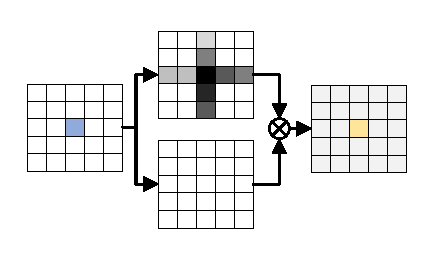
\includegraphics[width=0.7\linewidth]{figures/十字交叉注意力机制.pdf}
	\caption{十字交叉注意力机制}
	\label{fig:十字交叉注意力机制}
\end{figure}


将注意力模块加入到网络后,整体网络模型如图\ref{fig:整体网络}所示。
\begin{figure}[htbp]
	\centering
	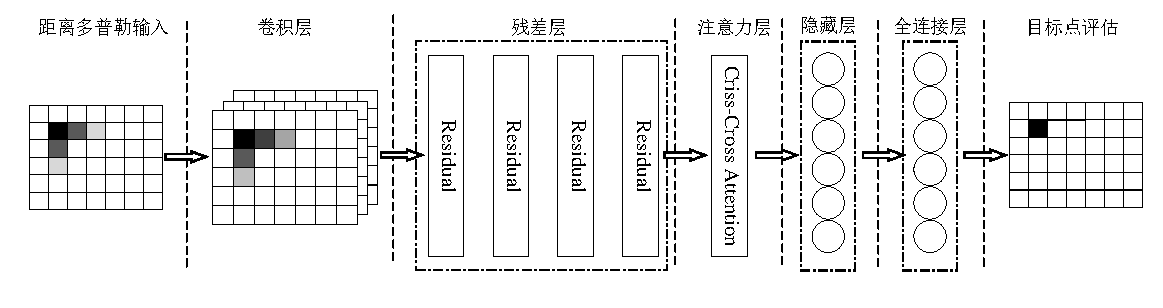
\includegraphics[width=\linewidth]{figures/整体网络.pdf}
	\caption{整体网络模型设计}
	\label{fig:整体网络}
\end{figure}

\subsection{训练流程}
(1)损失函数设计。本方案的输出结果为距离多普勒图中每一个单元是否有目标存在,可以抽象为对每个单元进行二分类问题。将单元格的输出视为概率,对每个单元格的输出结果与标签值,使用交叉熵损失函数用来衡量两个概率分布之间的距离。交叉熵损失函数的表达式如下:
\begin{equation}
	\label{eq:交叉熵损失函数}
	L(y,\hat{y}) = -\frac{1}{N}\sum_{i=1}^{N}y_i\log(\hat{y}_i) + (1-y_i)\log(1-\hat{y}_i)
\end{equation}
其中$y$为真实标签,$\hat{y}$为预测标签,$N$为样本数量。交叉熵损失函数的值越小,模型的预测结果越接近真实标签。

(2)优化器设计。在训练过程中,使用Adam优化器作为优化器。Adam优化器是一种自适应学习率的优化器,它可以根据每个参数的梯度自适应地调整学习率。Adam优化器的更新公式如\eqref{eq:Adam优化器}:
\begin{equation}
	\label{eq:Adam优化器}
	\begin{split}
		m_t &= \beta_1m_{t-1}+(1-\beta_1)g_t \\
		v_t &= \beta_2v_{t-1}+(1-\beta_2)g_t^2 \\
		\hat{m}_t &= \frac{m_t}{1-\beta_1^t} \\
		\hat{v}_t &= \frac{v_t}{1-\beta_2^t} \\
		\theta_{t+1} &= \theta_t - \frac{\alpha}{\sqrt{\hat{v}_t}+\epsilon}\hat{m}_t
	\end{split}
\end{equation}
其中$\beta_1$和$\beta_2$分别是梯度的一阶矩估计和二阶矩估计的指数衰减率,$\alpha$是学习率,$\epsilon$是为了数值稳定性而添加的小常数。

(3)训练过程中模型性能评估方式。在训练过程中不能直接只以准确率作为评价模型当前性能的指标,由于在距离多普勒图中,无目标点单元和有目标点单元分布不均匀,目标点单元占90\%以上,在判断时即使将所有的点判定为无目标,精确度也为90\%以上。为了正确评估训练过程中模型的性能,在本节除了准确率外还引入了精确率(Precission)、召回率(Recall),F1值作为性能评估指标\cite{goutte2005probabilistic}。目标点检测结果的分类如下:
\par TP(True Positive):真正例,有目标点单元检测为有目标点;
\par TN(True Negative):真反例,无目标点单元检测为无目标点;
\par FP(False Positive):假正例,无目标点单元检测为有目标点;
\par FN(False Positive):假反例,有目标点单元检测为无目标点。
\par 
精确率的含义为在模型检测出的有目标点数量占所有检测为有目标点数量的百分比,计算公式如下:
\begin{equation}
	\label{eq:精确率}
	Precision = \frac{TP}{TP+FP}
\end{equation}
召回率的含义为模型检测出的有目标点数量占所有目标点数量的百分比,计算公式如下:
\begin{equation}
	\label{eq:召回率}
	Recall = \frac{TP}{TP+FN}
\end{equation}
F1值是精确率和召回率的调和平均数,为了能够综合评价模型的性能,计算公式如下:
\begin{equation}
	\label{eq:F1值}
	F1 = \frac{2 \times Precision \times Recall}{Precision + Recall}
\end{equation}

(4)训练过程。使用交叉熵损失函数作为损失函数\cite{4767189},使用Adam优化器作为优化器,学习率为0.0001,批大小为8,训练的epoch数量为30。训练过程中将训练集分为训练集和验证集,训练集用来训练模型,验证集用来评估模型的性能。在每个epoch结束后,在验证集上评估模型的性能,使用Early Stopping策略\cite{yao2007early},当模型的性能没有提升时提前结束训练。训练过程中使用学习率衰减策略,当模型的性能没有提升时减小学习率。训率过程中的准确率、精确率、召回率、F1值曲线如图\ref{fig:RA-CFAR训练曲线}所示。

\begin{figure}[htbp]
	\centering
	\subcaptionbox{准确率(Accuracy)}{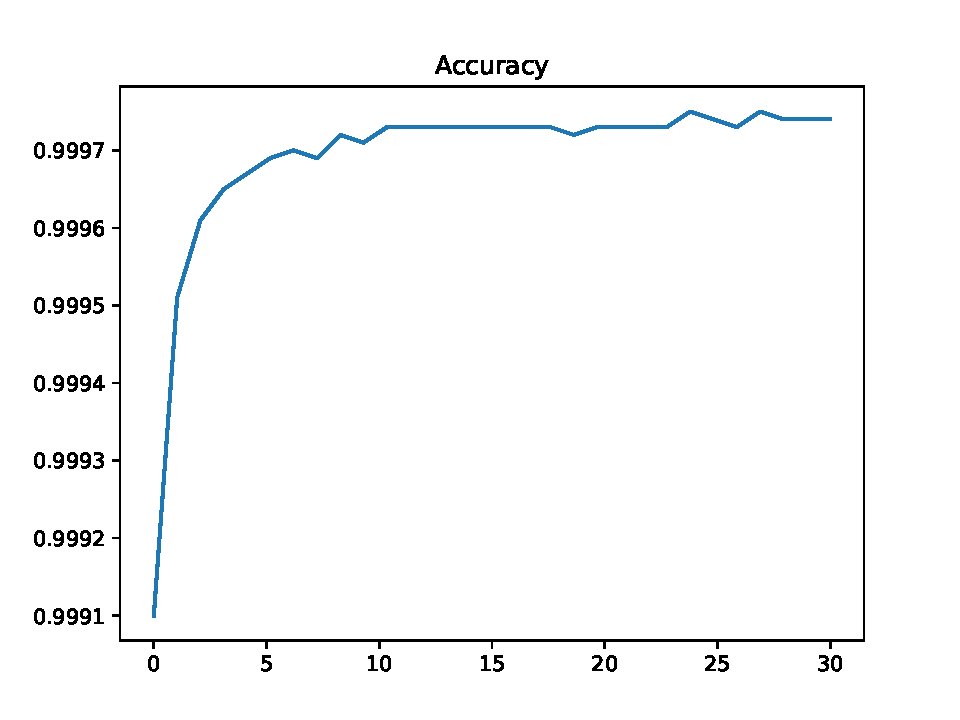
\includegraphics[width = 0.48\linewidth]{figures/准确率.pdf}}
	\subcaptionbox{精确率(Precision)}{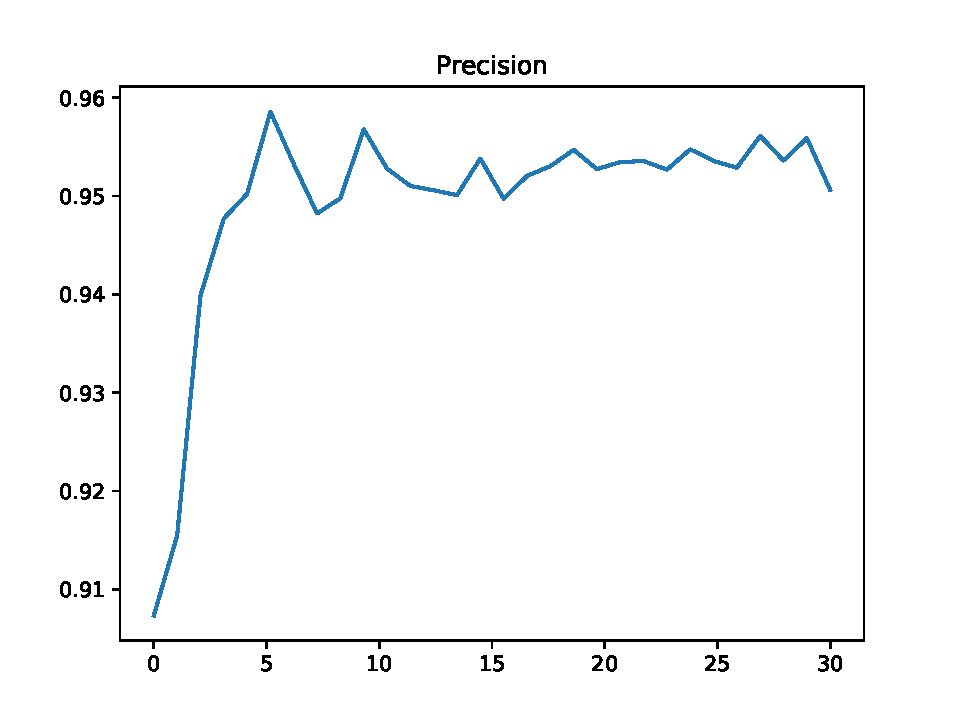
\includegraphics[width = 0.48\linewidth]{figures/精确率.pdf}}
	\subcaptionbox{召回率(Recall)}{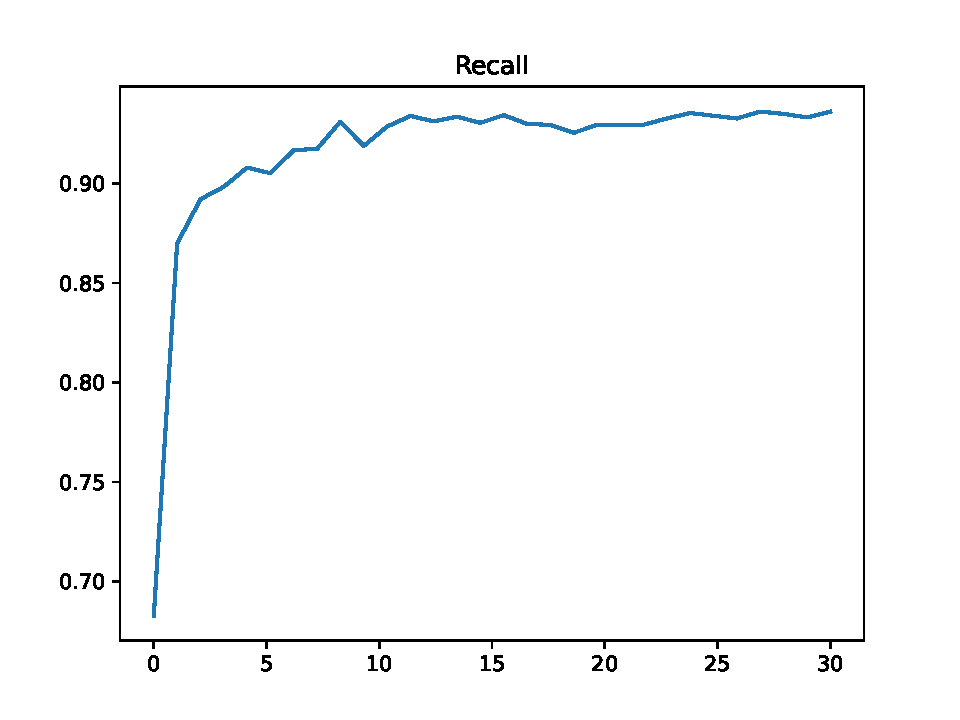
\includegraphics[width = 0.48\linewidth]{figures/召回率.pdf}}
	\subcaptionbox{F1值}{\includegraphics[width = 0.48\linewidth]{figures/F1值.pdf}}
	\caption{RA-CFAR训练曲线}
	\label{fig:RA-CFAR训练曲线}
\end{figure}


\section{实验设计与结果分析}
本节将RA-CFAR与其他几种常用的CFAR算法进行对比,通过对比实验结果分析RA-CFAR的性能。实验数据集为仿真数据集和实际采集的数据集。仿真数据集以\ref{训练数据生成}中同样的方式生成,采集数据集为\ref{实验数据采集}中数据集。实验评估指标为虚警率-检测率曲线和信噪比-检测率曲线。
\subsection{实验评估指标}
为了准确评估R-CFRA的性能,采用虚警率-检测率曲线在不同的信噪比下评估算法的性能。虚警率是指将背景噪声错误识别为目标的概率,检测率是正确识别目标点的比例。

对于输入的信号,可以用目标存在$H_0$和目标不存在$H_1$两个假设。假设$Z$为背景噪声的水平估计,$T$为参考门限因子,则$T \times Z$为门限值,当检测值$Y > T \times Z$,可以认为发现目标,反之没有目标。虚警率是在$H_0$的前提下,检测到目标。即可以表示为
$P(Y>TZ|H_0)$
由于噪声或杂波经过平方检波器后为指数分布,参考单元的概率密度函数为:
\begin{equation}
	f(x)=\frac{1}{2\mu}e^{-\frac{x}{2\mu}},x \ge 0
\end{equation}
从而得到虚警率的计算公式为:
\begin{equation}
	\begin{split}
			P_{fa} &= E \big( P(Y>TZ|H_0) \big) \\
			&= E_Z\big( \int_{T Z}^{\infty} f(y) d y \big)\\
			&= E_Z\big( \int_{T Z}^{\infty} \frac{1}{2\mu}e^{-\frac{y}{2\mu}} d y  \big)\\
			&= E_Z \big( e^{-\frac{TZ}{2\mu}} \big) \\
	\end{split}	
	\label{虚警率公式}
\end{equation}
\subsection{实验算法对比}
本节介绍了其他几种常用的CFAR算法,通过对比其他算法的表现分析算法性能。对比算法有CA-FAR、GOCA-CFAR、SOCA-CFAR、OS-CFAR。
\par
(1)CA-CFAR的背景杂波噪声计算公式是检测单元前后$N$个单元的平均值。
\begin{equation}
	Z_{CZ} = \frac{1}{N}\sum_{i=1}^{N}X_i
\end{equation}
计算门限因子的公式为:
\begin{equation}
	T_{CZ} = N(P^{\frac{1}{N}} - 1)
\end{equation}
\par
(2)GOCA-CFAR是选取检测单元前n个参考单元之和平均值与后n个参考单元之和平均值中大的作为背景杂波噪声评估水平。
\begin{equation}
	\begin{split}
		Y_1 &= \frac{1}{N} \sum_{n}^{i=1}X_i \\
		Y_2 &= \frac{1}{N} \sum_{2n}^{i=n+1}X_i\\
		Z_{GO} &= max\left(Y_1, Y_2\right)
	\end{split}
\end{equation}
计算门限因子需要使用递归方式,公式为:
\begin{equation}
	\begin{split}
	\frac{P_fa}{2} &= \left(1+\frac{T_{GO}}{n} \right)^{-n} -   \left(2+\frac{T_{GO}}{n} \right)^{-n} 
	\cdot  \left\{ \sum_{i=0}^{n-1}\begin{pmatrix}  n+i-1\\i \end{pmatrix} \left(2+ \frac{T_{GO}}{n} \right)^{-k} \right\} \\
	P_fa &= 2\left( 1+T \right)^{-n} -  2\sum_{i=0}^{n-1}\begin{pmatrix}  n+i-1\\i \end{pmatrix}  \left(2+T_{GO} \right)^{-(n+i)}
	\end{split}
\end{equation}
\par
(3)SOCA-CFAR是选取检测单元前n个参考单元之和平均值与后n个参考单元之和平均值中小的作为背景杂波噪声评估水平。
\begin{equation}
	\begin{split}
		Y_1 &= \frac{1}{N} \sum_{n}^{i=1}X_i \\
		Y_2 &= \frac{1}{N} \sum_{2n}^{i=n+1}X_i\\
		Z_{GO} &= min\left(Y_1, Y_2\right)
	\end{split}
\end{equation}
计算门限因子需要使用递归方式,公式为:
\begin{equation}
	\begin{split}
		\frac{P_fa}{2} &=  \left(2+\frac{T_{GO}}{n} \right)^{-n} 
		\cdot  \left\{ \sum_{i=0}^{n-1}\begin{pmatrix}  n+i-1\\i \end{pmatrix} \left(2+ \frac{T_{GO}}{n} \right)^{-k} \right\} \\
		P_fa &= 2\sum_{i=0}^{n-1}\begin{pmatrix}  n+i-1\\i \end{pmatrix}  \left(2+T_{GO} \right)^{-(n+i)}
	\end{split}
\end{equation}
\par
(4)OS-CFAR是先将检测单元排序,选取第$k$个样本作为背景杂波评估水平。
\begin{equation}
	\begin{split}
		Y_1 &= \frac{1}{N} \sum_{n}^{i=1}X_i \\
		Y_2 &= \frac{1}{N} \sum_{2n}^{i=n+1}X_i\\
		Z_{GO} &= min\left(Y_1, Y_2\right)
	\end{split}
\end{equation}
可以使用递归方式计算门限因子,公式为:
\begin{equation}
	P_fa = k \begin{pmatrix}  2n \\k \end{pmatrix} \frac{\left( k-1\right)! \left(T_{OS} + 2n-k \right)! }{\left( T_{OS} + 2n \right)!}
\end{equation}
\par

\subsection{结果分析}
通过比较本章提出RA-CFAR和其他四种CFAR算法的表现,进行实验效果的评估。
\par
(1) 在不同信噪比(本节选择20、25、30、35dB)目标数量(1到3)均匀分布,各个算法检测率随虚警率变化如图\ref{fig:多个SNR检测率}所示。在多个信噪比下,RA-CFAR的虚警率-检测率曲线均优于其他方案。
\begin{figure}[htbp]
	\centering
	\subcaptionbox{SNR=20dB}{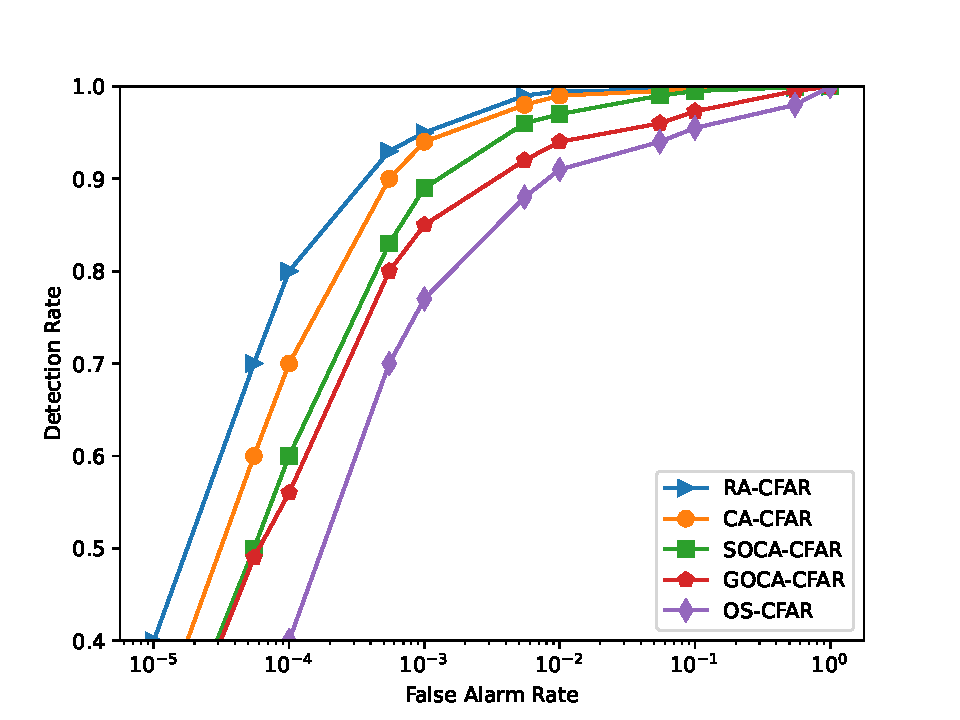
\includegraphics[width = 0.48\linewidth]{figures/20_snr.pdf}}
	\subcaptionbox{SNR=25dB}{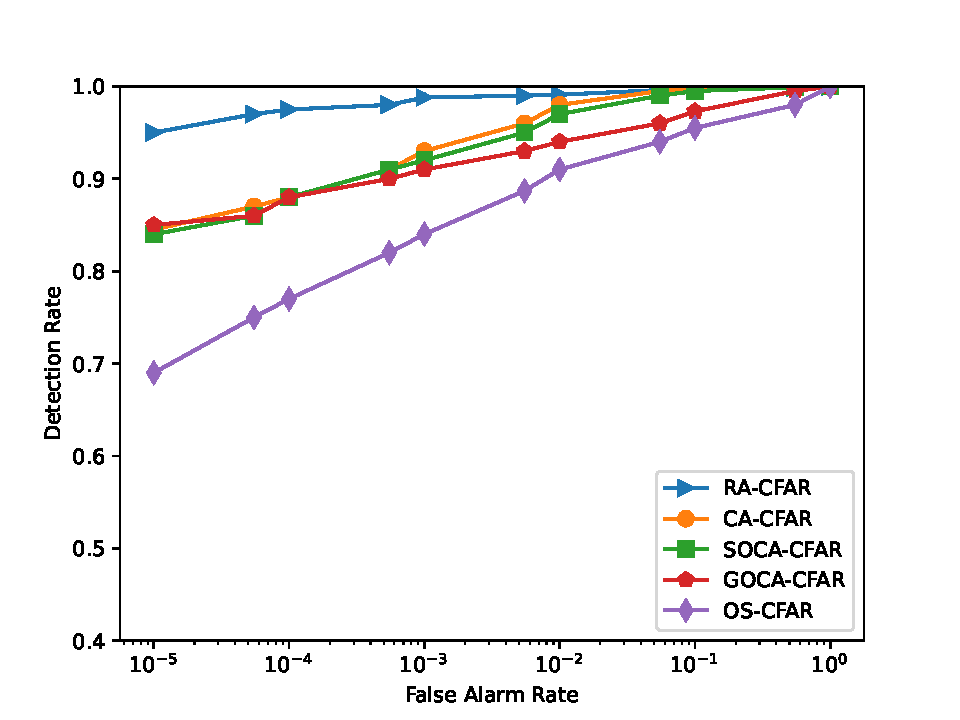
\includegraphics[width = 0.48\linewidth]{figures/25_snr.pdf}}
	\subcaptionbox{SNR=30dB}{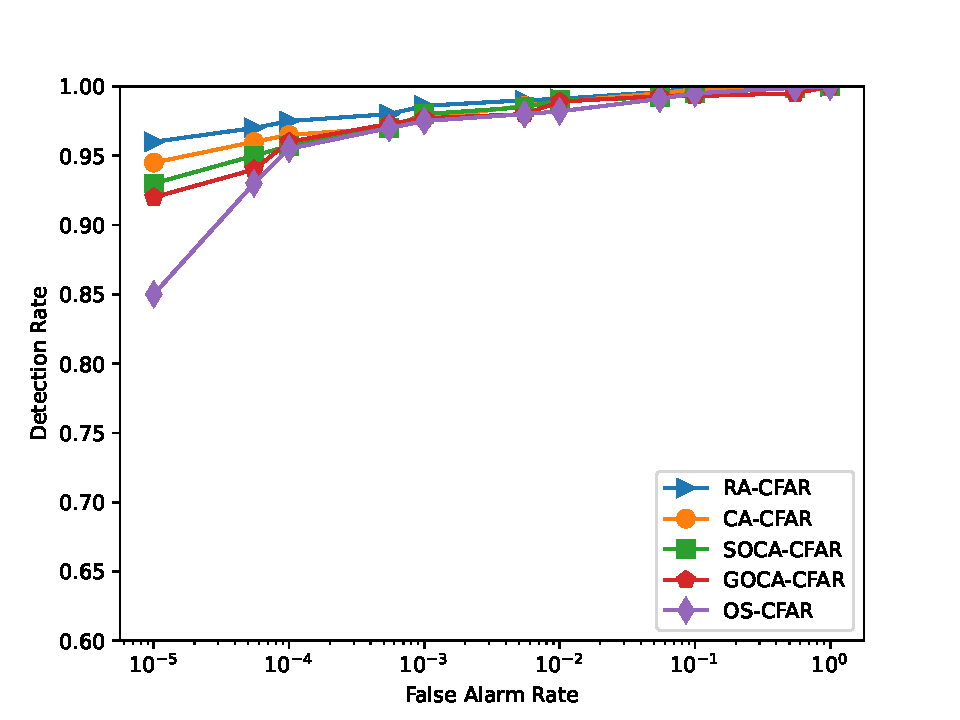
\includegraphics[width = 0.48\linewidth]{figures/30_snr.pdf}}
	\subcaptionbox{SNR=35dB}{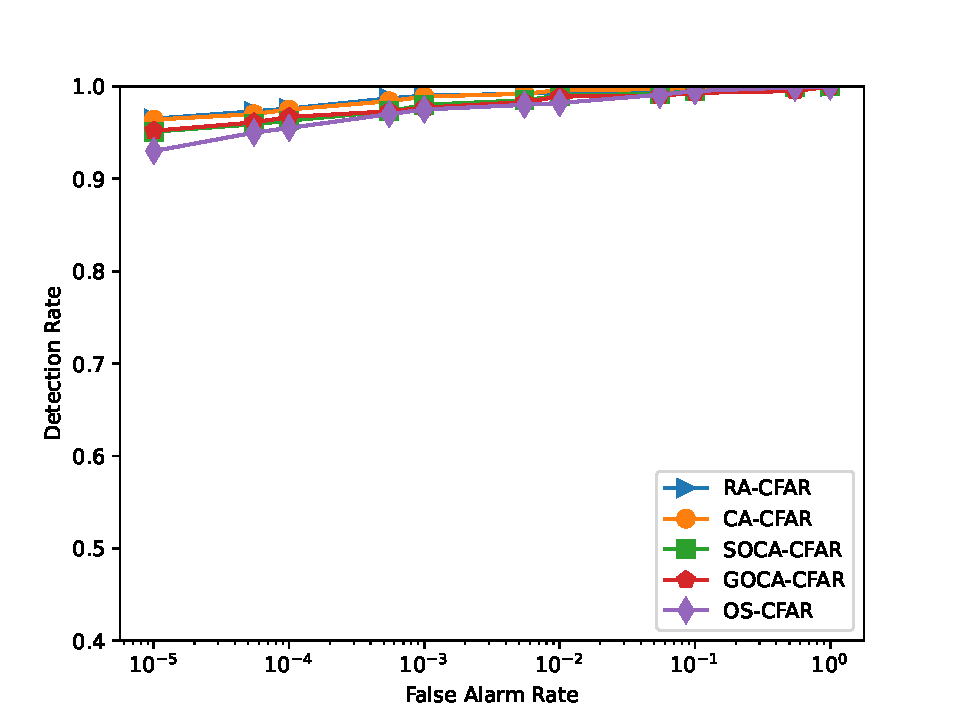
\includegraphics[width = 0.48\linewidth]{figures/35_snr.pdf}}
	\caption{多个信噪比下检测率}
	\label{fig:多个SNR检测率}
\end{figure}
\par
为了直观体现性能对比,计算出每条虚警率-检测率曲线下的面积(Area Under Curve,AUC),在各个信噪比下AUC值如表\ref{多信噪比AUC}所示,RA-CFAR在多数情况下取得了良好的效果,在低信噪比的情况下(20dB)相比于其他四种算法AUC值分别提升了4\%、8\%、11.9\%、29.4\%。在信噪比较高的情况下检测效果也与CA-CFAR相当。对比AUC值RA-CFAR在20、25、30dB的情况下均取得了最好的成绩,而在35dB的情况下效果仅次于CA-CFAR,其原因可能是在高信噪比的情况下目标与背景之间的差异更加显著,从而使得目标检测更容易。
\begin{table}[htbp]
	\centering
	\tabcolsep=2mm
	\caption{多信噪比AUC}
	\begin{tabular}{cccccc}
		\toprule
		噪声 & CA-CFAR  & SOCA-CFAR & GOCA-CFAR&OS-CFAR& \textbf{RA-CFAR} \\
		\midrule
		20dB & 0.852 & 0.815 & 0.792 & 0.685 & \textbf{0.887}\\
		25dB & 0.941 & 0.938 & 0.927 & 0.863 & \textbf{0.985} \\
		30dB & 0.980 & 0.973 & 0.975 & 0.966 & \textbf{0.986}\\
		35dB & \textbf{0.987} & 0.979 & 0.980 & 0.975 & 0.986\\
		\bottomrule
	\end{tabular}
	\label{多信噪比AUC}
\end{table}


(2)在相同的虚警率下,检测率随信噪比变化。如图\ref{fig:检测率随信噪比变化}
\begin{figure}[htbp]
	\centering
	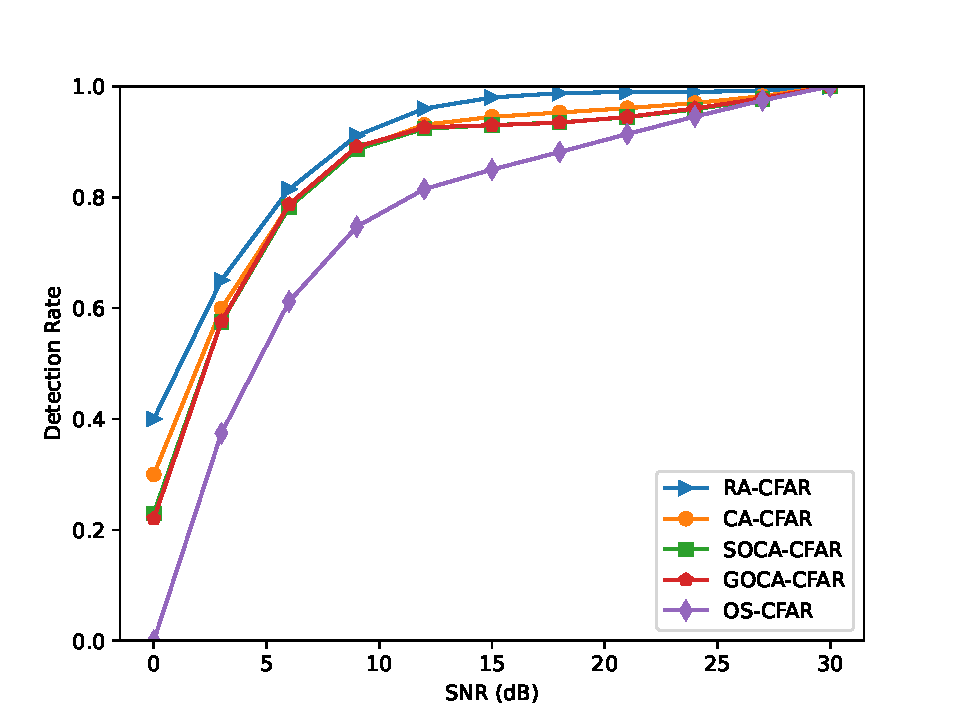
\includegraphics[width = 0.6\linewidth]{figures/检测率随信噪比变化.pdf}
	\caption{检测率随信噪比变化}
	\label{fig:检测率随信噪比变化}
\end{figure}
可以看出随着信噪比的增大使目标检测难度变小,所有的算法检测率表现都在变好,但是在低信噪比的情况下RA-CFAR具有明显的优势,当信噪比逐渐增大时RA-CFAR的效果仍优于其他算法。

\begin{figure}[htbp]
	\centering
	\subcaptionbox{SNR=25dB,1目标}{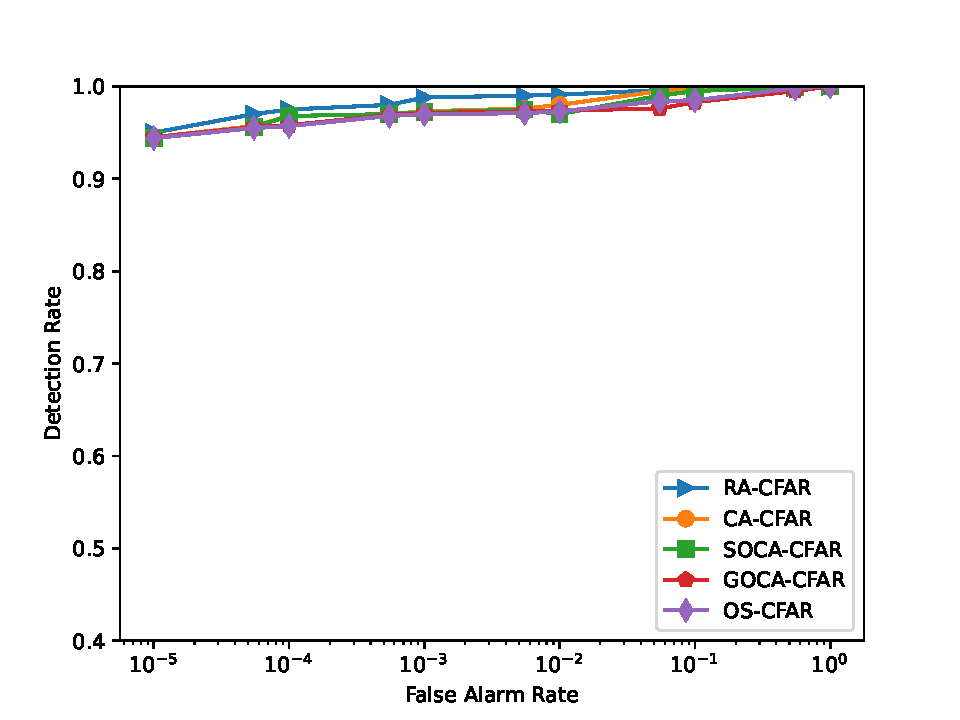
\includegraphics[width = 0.45\textwidth]{figures/1目标.pdf}}
	\subcaptionbox{SNR=25dB,2目标}{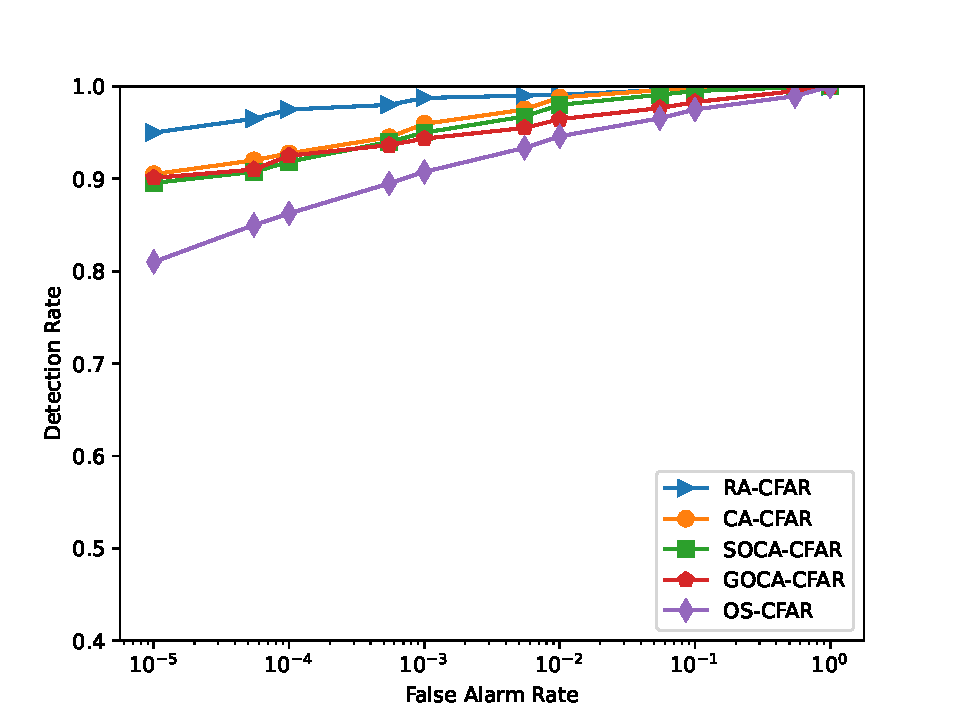
\includegraphics[width = 0.45\textwidth]{figures/2目标.pdf}}
	\subcaptionbox{SNR=25dB,3目标}{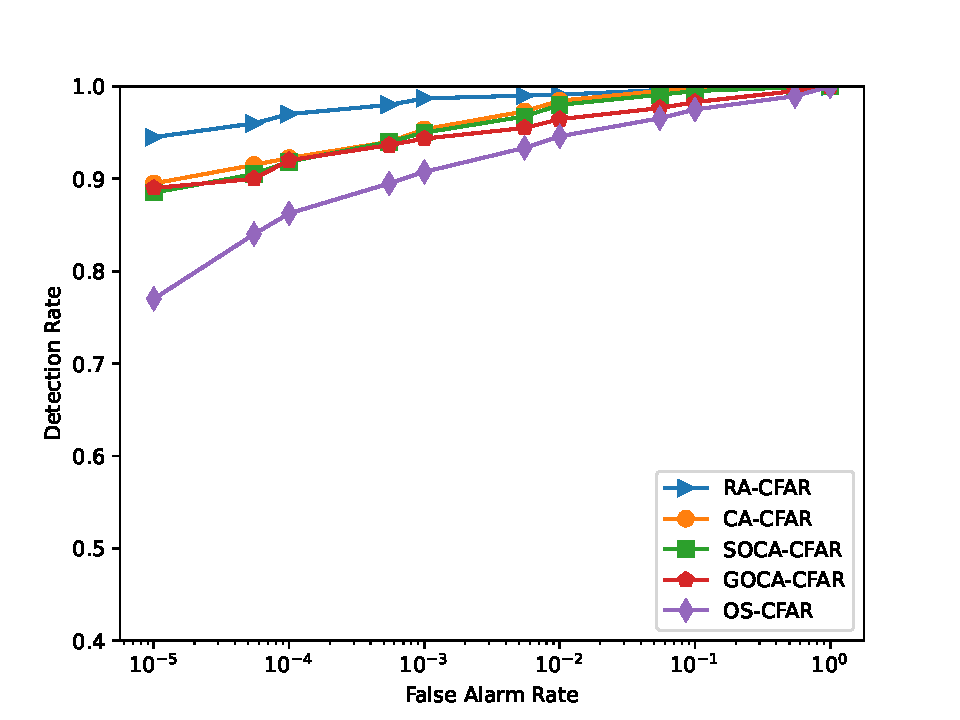
\includegraphics[width = 0.45\textwidth]{figures/3目标.pdf}}

	\caption{不同目标数量检测率对比}
	\label{fig:不同目标数量检测率对比}
\end{figure}
\begin{table}[htbp]
	\centering
	\tabcolsep=2mm
	\caption{多目标数量AUC}
	\begin{tabular}{cccccc}
		\toprule
		目标数 & CA-CFAR  & SOCA-CFAR & GOCA-CFAR&OS-CFAR& \textbf{RA-CFAR} \\
		\midrule
		1 & 0.978 & 0.976 & 0.973 & 0.973 & \textbf{0.985}\\
		2 & 0.965 & 0.959 & 0.954 & 0.921 & \textbf{0.985} \\
		3 & 0.961 & 0.957 & 0.951 & 0.917 & \textbf{0.983}\\
		\bottomrule
	\end{tabular}
	\label{多目标数量AUC}
\end{table}


(3)在相同的信噪比下,不同目标数量检测率随虚警率变化。为了比较各个算法在不同目标数量时的性能,在本节将SNR固定为25dB,检测各个算法在25dB下不同人数的检测率随虚警率变化。由图\ref{fig:不同目标数量检测率对比}可知,当多目标时其他算法的检测率都出现明显的下降,只有RA-CFAR的检测率仍然保持相对稳定,当目标数量为3时,对比其他算法AUC值分别提升了2.29\%、2.71\%、3.36\%、7.19\%。

\begin{figure}[htbp]
	\centering
	\subcaptionbox{距离多普勒三维视图\label{距离多普勒三维视图}}{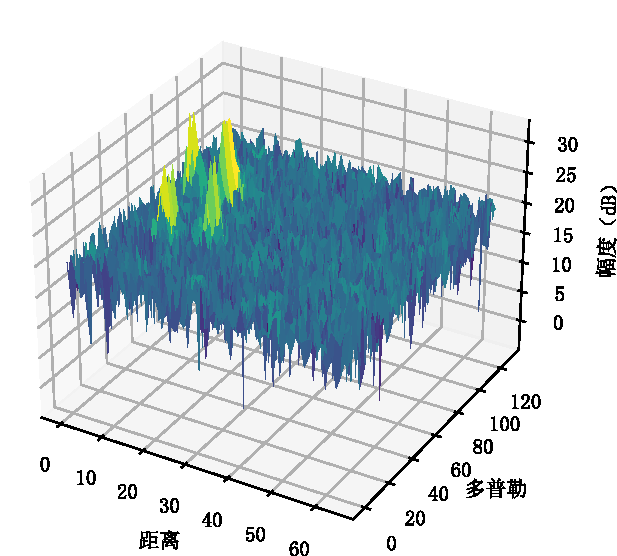
\includegraphics[width = 0.45\linewidth]{figures/4目标/距离多普勒3d.pdf}}
	\subcaptionbox{距离多普勒图\label{距离多普勒图}}{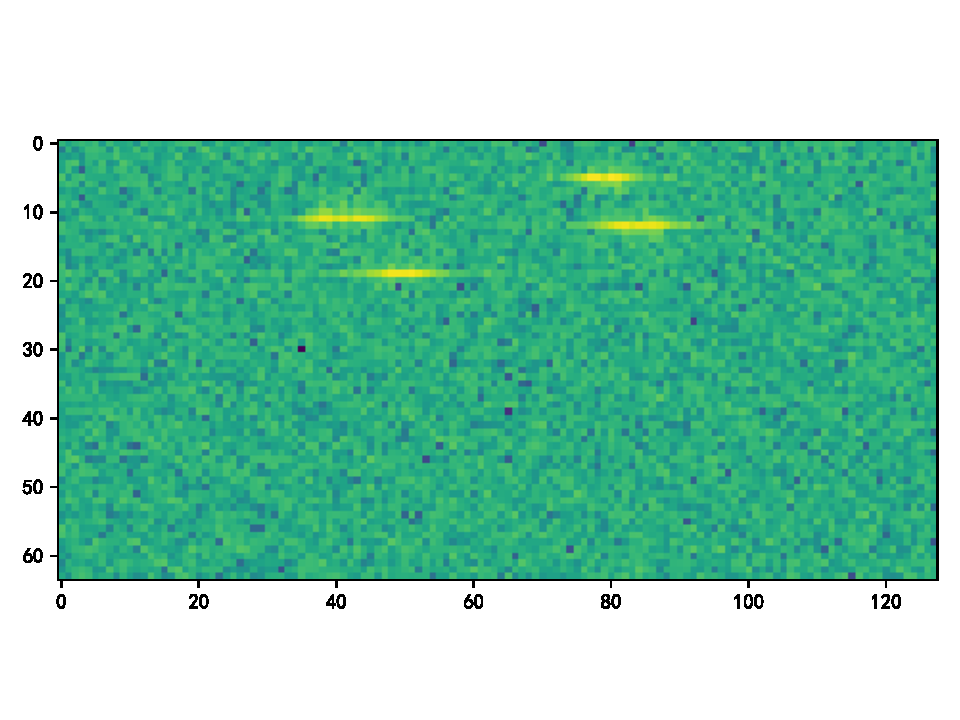
\includegraphics[width = 0.45\linewidth]{figures/4目标/距离多普勒2d.pdf}}
	\caption{四目标距离多普勒图}
	\label{fig:四目标距离多普勒图}
\end{figure}

(4)为验证模型的泛化性,使用在训练集没有出现过的4目标场景进行测试。距离多普勒图如图\ref{fig:四目标距离多普勒图},RA-CFAR检测结果如图\ref{RA-CFAR三维视图}所示,目标点实际分布如图\ref{目标点三维视图}所示。由图可知RA-CFAR在4目标检测场景下仍然保持了较好的检测效果,能够有效地检测出目标点。

\begin{figure}[htbp]
	\centering
	\subcaptionbox{RA-CFAR三维视图\label{RA-CFAR三维视图}}{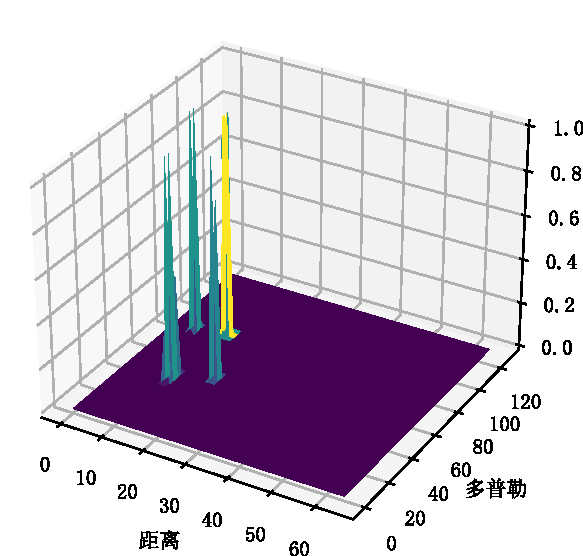
\includegraphics[width = 0.45\linewidth]{figures/4目标/RA-CFAR3d.pdf}}
	\subcaptionbox{RA-CFAR\label{RA-CFAR}}{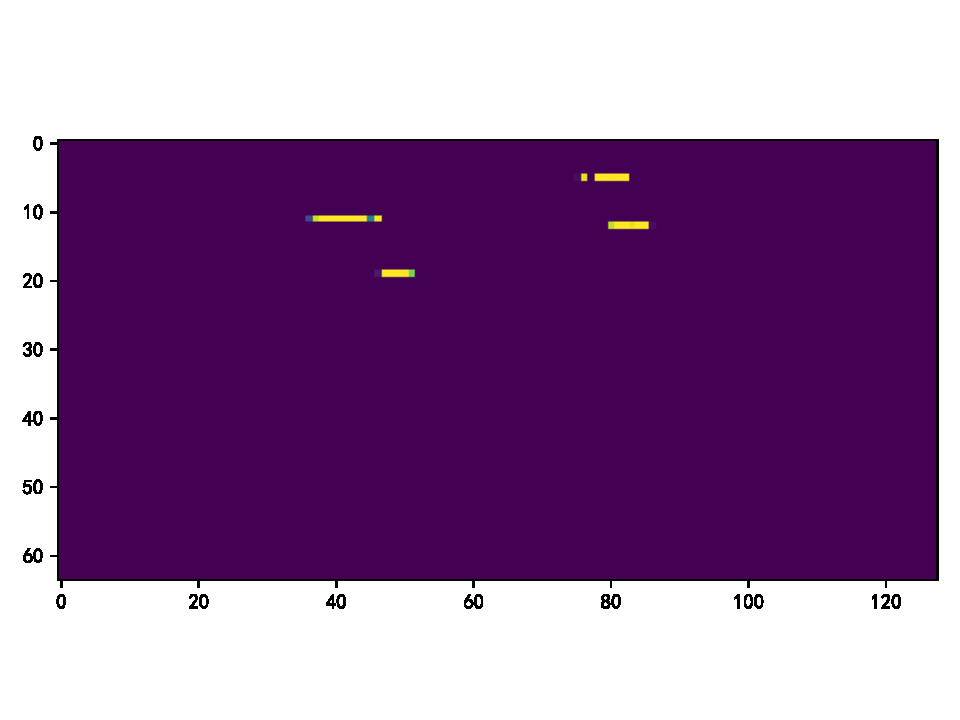
\includegraphics[width = 0.45\linewidth]{figures/4目标/RA-CFAR2d.pdf}}
	\subcaptionbox{目标点三维视图\label{目标点三维视图}}{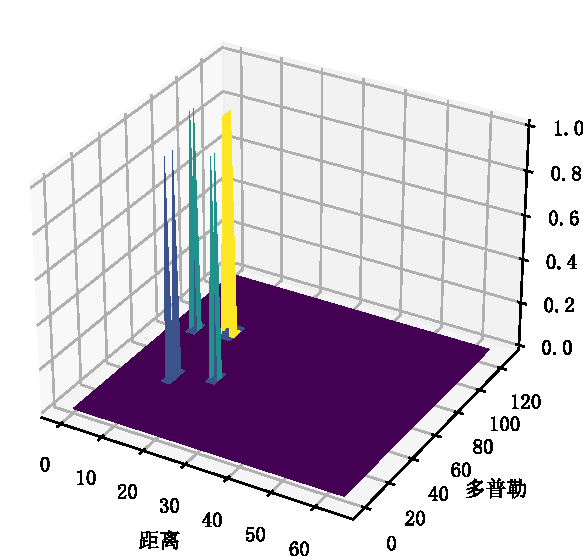
\includegraphics[width = 0.45\linewidth]{figures/4目标/gt3d.pdf}}
	\subcaptionbox{目标点\label{目标点}}{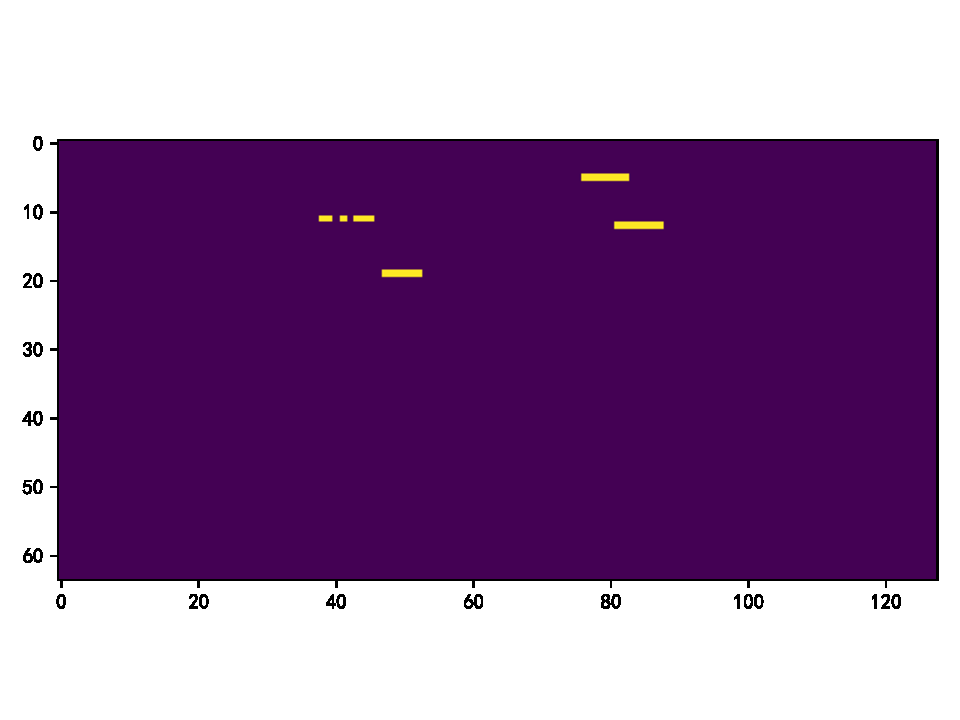
\includegraphics[width = 0.45\linewidth]{figures/4目标/gt2d.pdf}}
	\caption{四目标检测结果}
	\label{fig:四目标检测结果}
\end{figure}

\section{本章小结}
本章分析了当前CFAR算法的问题,发现在大多数情况下CA-CAFR等经典算法,可以有效的检测出目标点。但是面对多目标和较低信噪比情景下存在性能下降以及难以设置参数的问题。而残差神经网络和注意力机制,能够有效地提取和学习不同位置的距离多普勒图的空间特征关联信息,可以准确排除噪声干扰检测出目标点。因此,本章基于此方案设计了基于残差神经网络和十字交叉注意力模块的RA-CFAR方案,与CA-FAR、GOCA-CFAR、SOCA-CFAR、OS-CFAR在多个数据集上进行了对比实验,验证了RA-CFAR方案的有效性。


